\documentclass[a4paper]{article}
\usepackage[margin = 1 in]{geometry}
\usepackage{fancyhdr}
\usepackage{lastpage}
\usepackage{ctex}
\usepackage[utf8]{inputenc} % Required for inputting international characters
\usepackage[T1]{fontenc} % Output font encoding for international characters
\usepackage[sfdefault]{ClearSans} % Use the Clear Sans font (sans serif)
\usepackage{tocloft} 
\usepackage[hidelinks]{hyperref}
\usepackage{makecell}%导入表格宏包
\usepackage{bmpsize}
\usepackage{graphicx}
\usepackage{epstopdf}
\usepackage{caption}
\usepackage{enumitem}
\usepackage{float}
\usepackage{multirow}
\usepackage{makecell}

\pagestyle{fancy}
\lhead{\textsl{Final Year Project}}
\chead{}
\rhead{Page \thepage\ of \pageref{LastPage}}
\lfoot{}
\rfoot{}
\cfoot{}
\renewcommand{\headrulewidth}{0.4pt}
\renewcommand{\footrulewidth}{0pt}
\renewcommand{\cftsecleader}{\cftdotfill{\cftdotsep}}
\newcommand{\tabincell}[2]{\begin{tabular}{@{}#1@{}}#2\end{tabular}} %单元格内换行

\renewcommand*\contentsname{Table of Contents}

\begin{document}

%----------------------------------------------------------------------------------------
%	TITLE PAGE
%----------------------------------------------------------------------------------------

\begin{titlepage}
	
	\rule{\linewidth}{5pt}
	\raggedleft
	\fontsize{38pt}{50pt}\selectfont
    \textbf{\\Team Project\\}
    \fontsize{28pt}{60pt}\selectfont 
    for\\
    \fontsize{38pt}{60pt}\selectfont 
    \textbf{Milestone 1\\}
	
	\vfill % Space between the title box and author information
	
	%------------------------------------------------
	%	Author name and information
	%------------------------------------------------
	
	\parbox[t]{0.93\textwidth}{ % Box to inset this section slightly
		\raggedleft % Right align the text
		\large % Increase the font size
		{\Large By Zijun Li\_2272583\_zxl183}\\[4pt] % Extra space after name
	}
	
\end{titlepage}

\begin{center}
	\tableofcontents
	\addcontentsline{toc}{section}{Table of Contents}
\end{center}
\newpage

\section{Agreed, coherent project concept \& personas \& mockups}

\subsection{Project concept}

In the digital age, where information overload is a common issue, the ability to skim through news without missing essential content becomes crucial. "Mirror News Summarizer" serves this need by offering users a streamlined version of their favorite news portals with the added advantage of concise summaries, allowing for efficient consumption of news. Recognizing the diverse interests of readers and the importance of personalization, we aim to take this platform a step further by integrating a sophisticated recommendation page. This unique feature stands to revolutionize the user experience by curating news articles based on popularity and user interaction within the mirrored sites, all housed within a separate, dedicated page.

\begin{enumerate}[wide, labelwidth=!, labelindent=0pt, label=\textbf{\arabic*.}]
    \item \textbf{Quick News Overview}: 
    Users can swiftly get the gist of articles through intelligent summarization, allowing them to consume more information in less time. Each piece retains key points and facts, ensuring a comprehensive understanding without the need for full-length reading.

    \item \textbf{Familiar Interface Design}: 
    The mirror aspect maintains the original website design, providing a comfortable and familiar browsing experience. Users navigate as usual, but with the benefit of quick, summarized content.

    \item \textbf{Personalized Recommendations}: 
    A dedicated page offers users a list of articles resonating with a wider audience, powered by real-time analysis of clicks and reads across the platform. It’s not just what’s trending globally; it’s what like-minded individuals are reading.

    \item \textbf{Interest-Based Curation}:
    Over time, the system learns from individual user interactions, allowing for a more tailored article suggestion list that aligns with their reading preferences and interests.

    \item \textbf{Engagement Through Feedback}:
    Users have the opportunity to react to summaries and recommended articles, providing feedback that enhances and personalizes their news consumption journey. This input directly influences future summarization and recommendation quality.
\end{enumerate}

\subsection{mockups}

\subsubsection{Scheduler}

\begin{figure}[H] %H为当前位置,!htb为忽略美学标准,htbp为浮动图形
	\centering %图片居中
	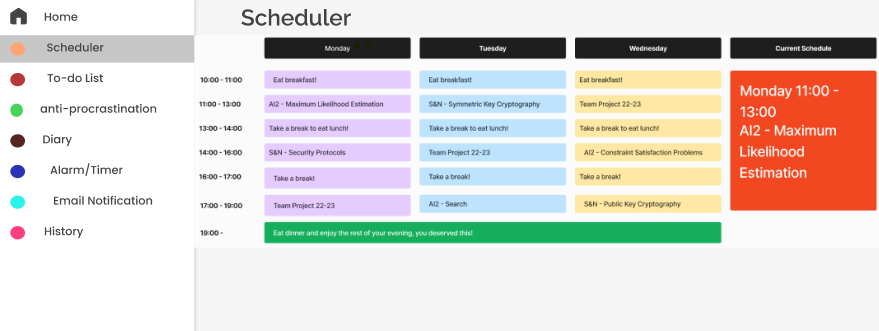
\includegraphics[width=1\textwidth]{./images/Mockup_Scheduler.png} %插入图片,[]中设置图片大小,{}中是图片文件名
	\caption*{Mockup: Scheduler} %最终文档中希望显示的图片标题
	\label{Fig.Scheduler} %用于文内引用的标签
\end{figure}

\subsubsection{To-do List}

\begin{figure}[H] %H为当前位置,!htb为忽略美学标准,htbp为浮动图形
	\centering %图片居中
	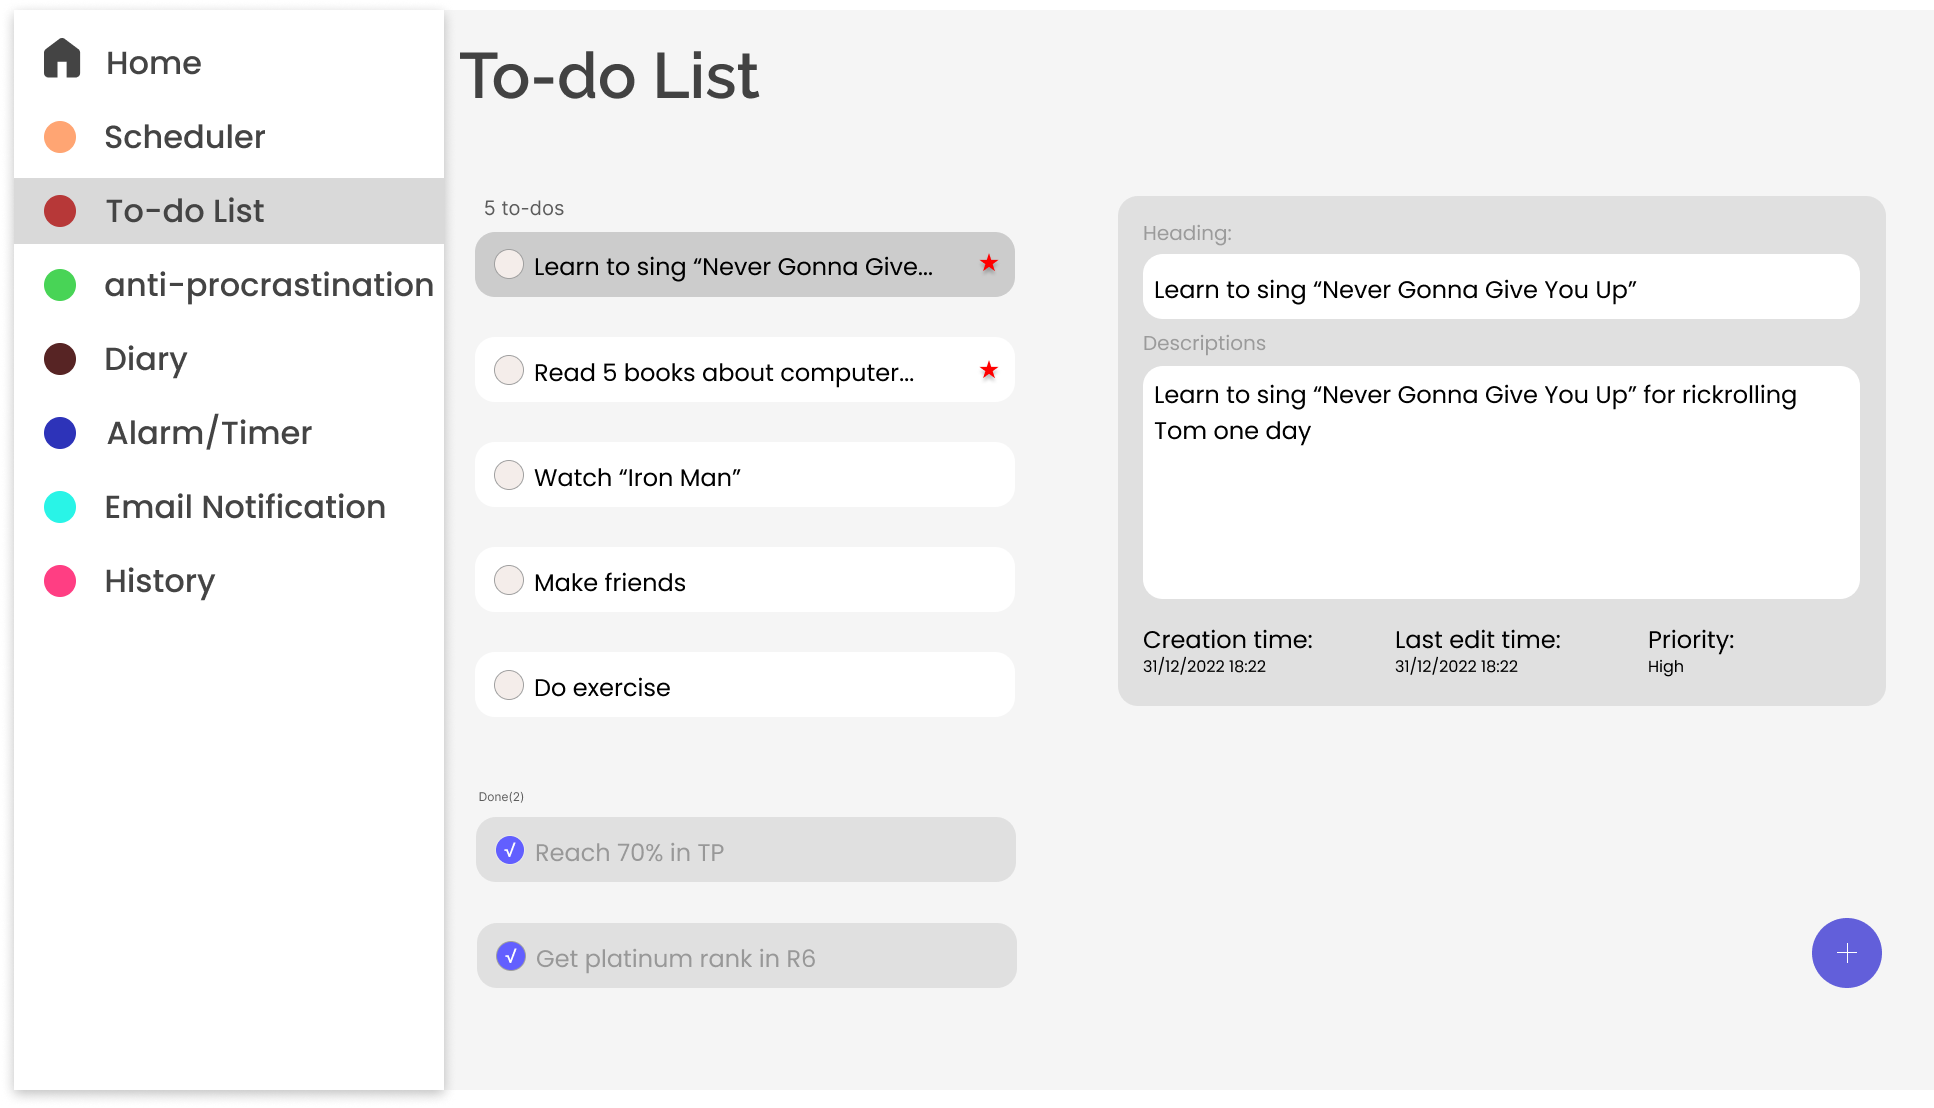
\includegraphics[width=1\textwidth]{./images/Mockup_Todo_list.png} %插入图片,[]中设置图片大小,{}中是图片文件名
	\caption*{Mockup: To-do List} %最终文档中希望显示的图片标题
	\label{Fig.todolist} %用于文内引用的标签
\end{figure}


\subsubsection{Anti-procrastination}

\begin{figure}[H] %H为当前位置,!htb为忽略美学标准,htbp为浮动图形
	\centering %图片居中
	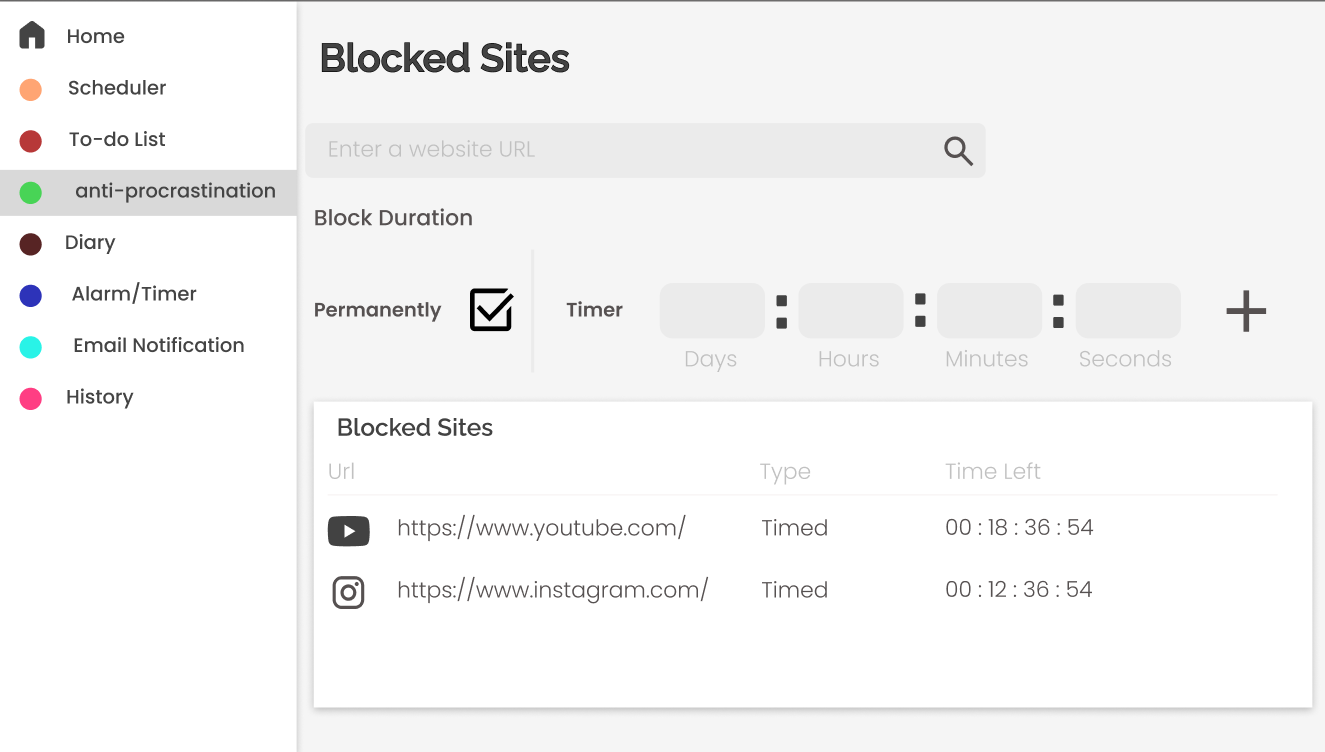
\includegraphics[width=1\textwidth]{./images/Mockup_Anti-procrastination.png} %插入图片,[]中设置图片大小,{}中是图片文件名
	\caption*{Mockup: Anti-procrastination} %最终文档中希望显示的图片标题
	\label{Fig.Anti-procrastination} %用于文内引用的标签
\end{figure}

\subsubsection{Diary}

\begin{figure}[H] %H为当前位置,!htb为忽略美学标准,htbp为浮动图形
	\centering %图片居中
	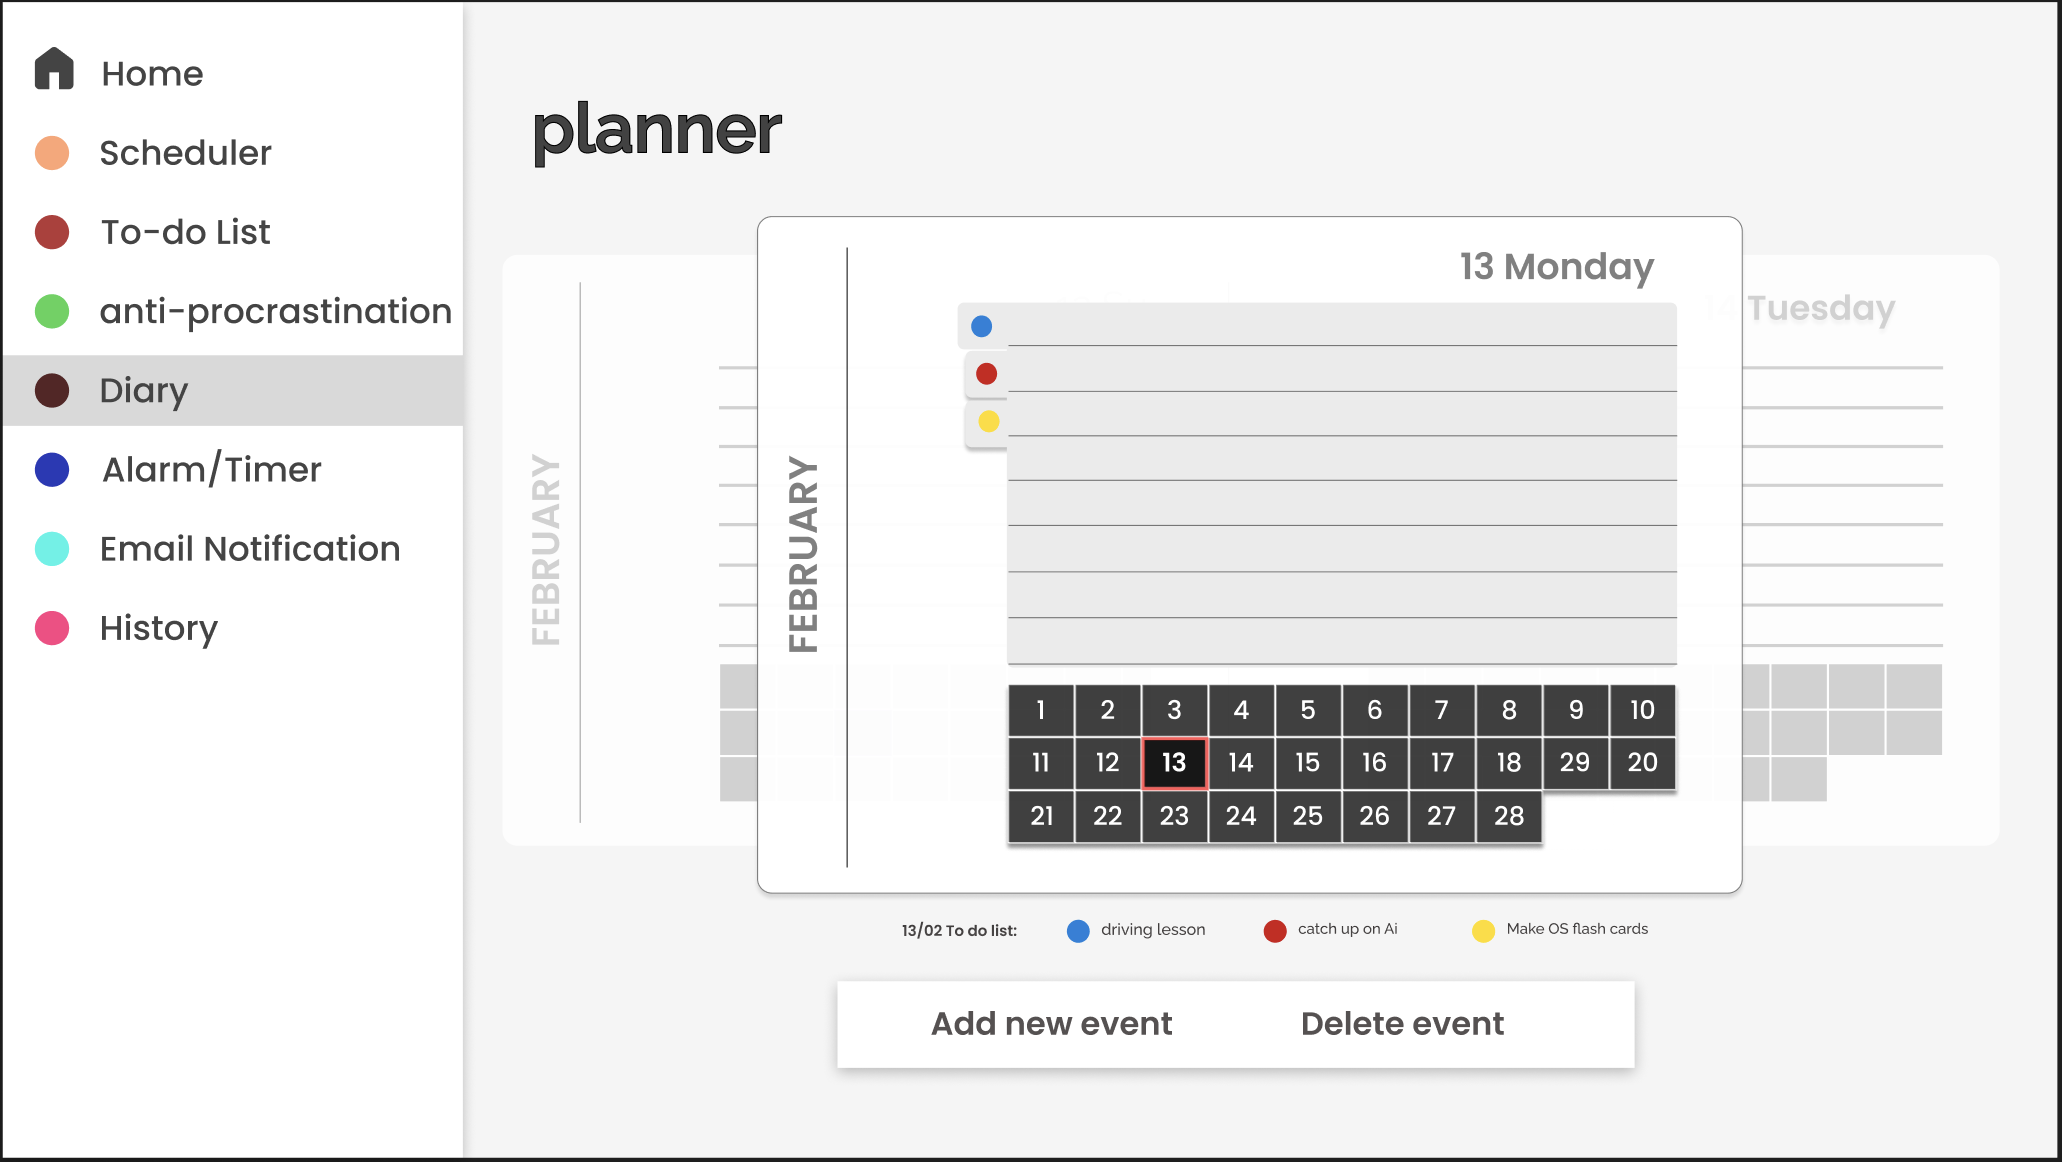
\includegraphics[width=1\textwidth]{./images/Mockup_Diary.jpg} %插入图片,[]中设置图片大小,{}中是图片文件名
	\caption*{Mockup: Diary} %最终文档中希望显示的图片标题
	\label{Fig.Diary} %用于文内引用的标签
\end{figure}

\subsubsection{Alarm/Timer}

\begin{figure}[H] %H为当前位置,!htb为忽略美学标准,htbp为浮动图形
	\centering %图片居中
	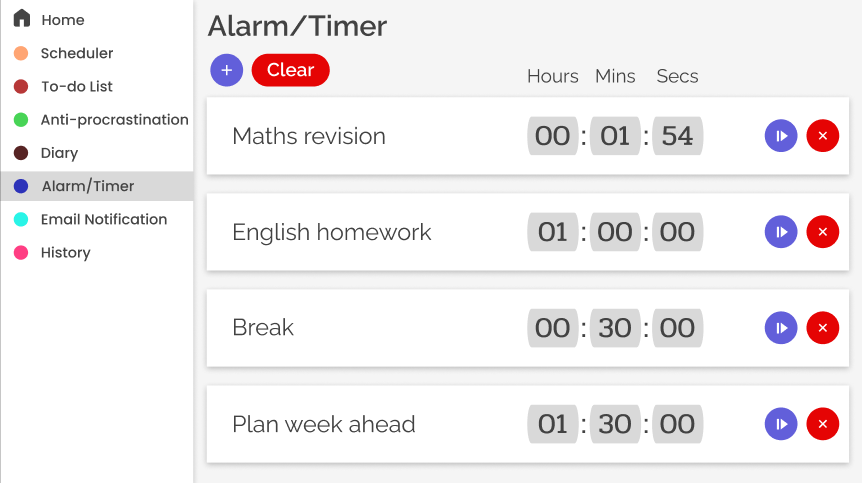
\includegraphics[width=1\textwidth]{./images/Mockup_AlarmTimer.png} %插入图片,[]中设置图片大小,{}中是图片文件名
	\caption*{Mockup: Alarm} %最终文档中希望显示的图片标题
	\label{Fig.Alarm} %用于文内引用的标签
\end{figure}

\subsubsection{History}

\begin{figure}[H] %H为当前位置,!htb为忽略美学标准,htbp为浮动图形
	\centering %图片居中
	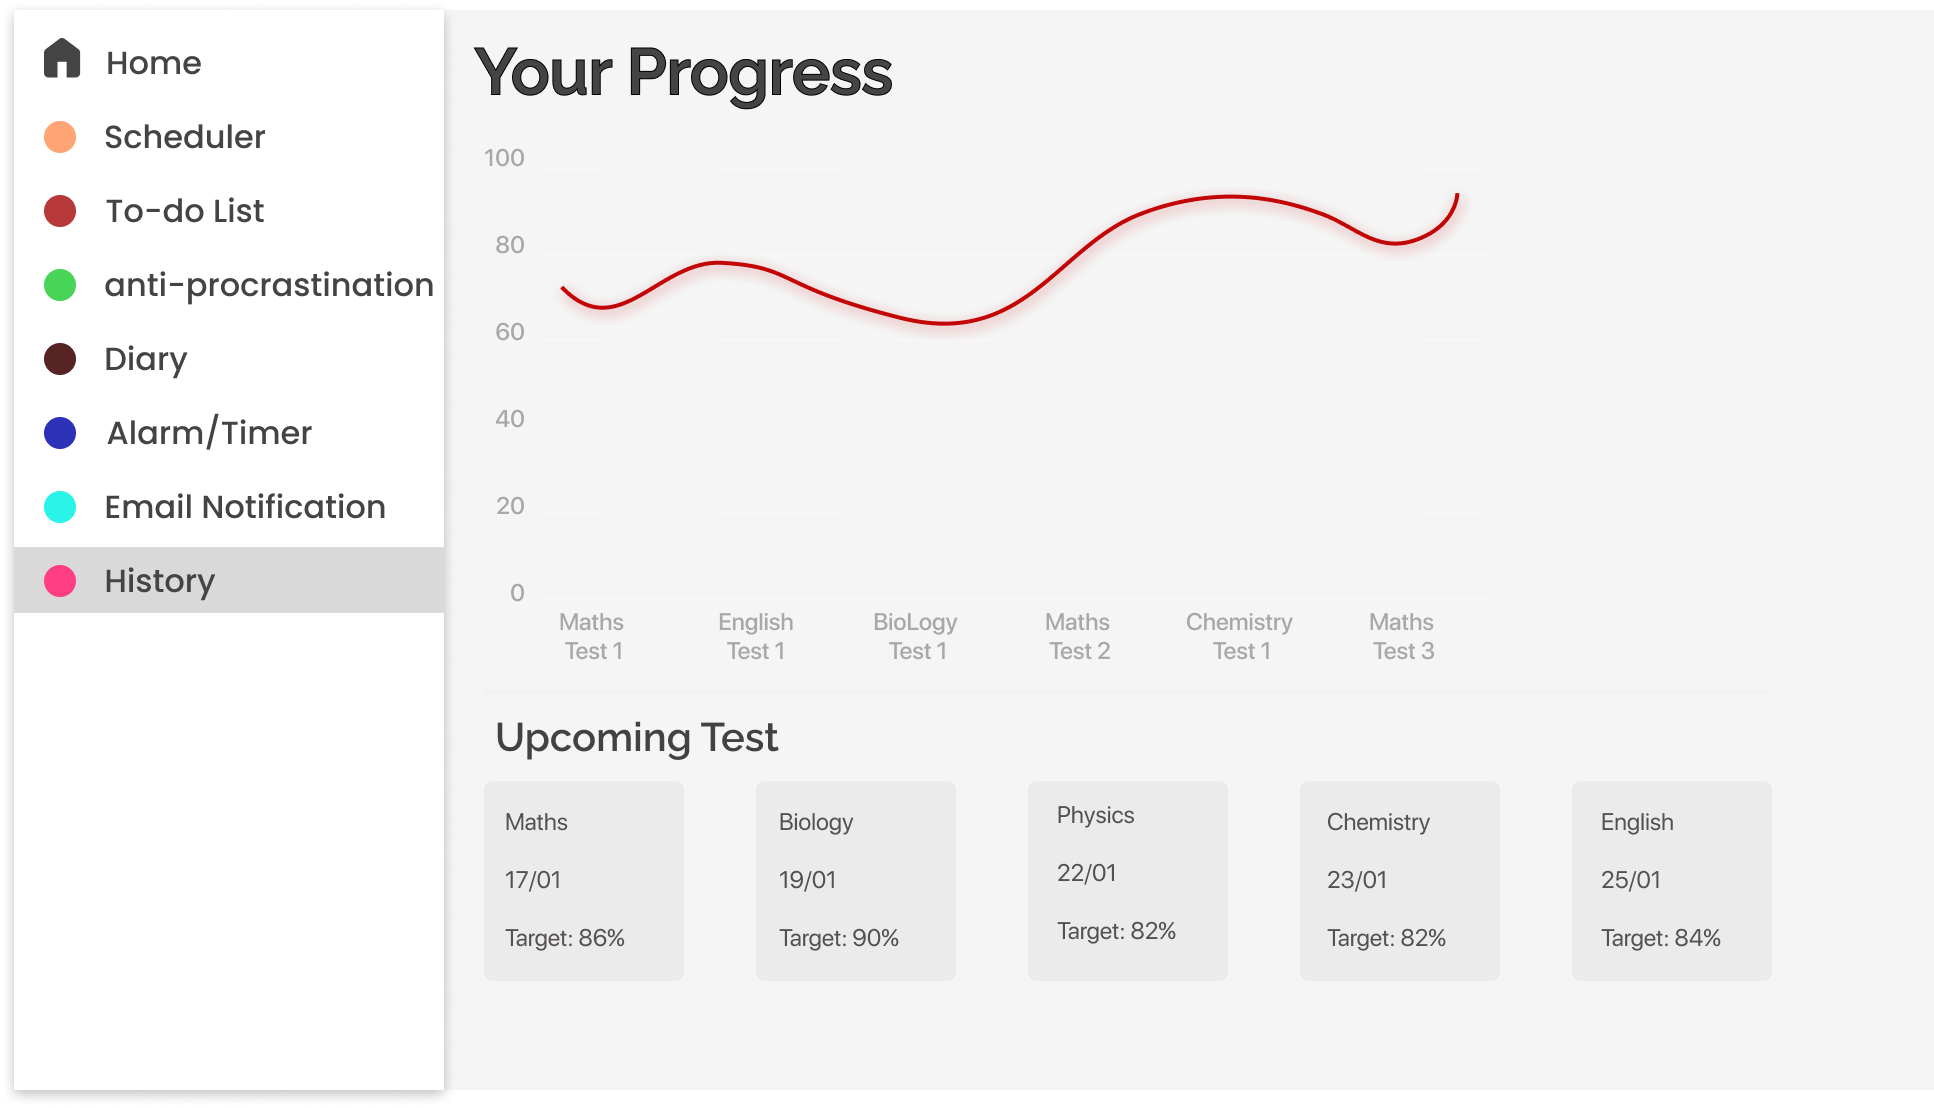
\includegraphics[width=1\textwidth]{./images/Mockup_History.png} %插入图片,[]中设置图片大小,{}中是图片文件名
	\caption*{Mockup: History} %最终文档中希望显示的图片标题
	\label{Fig.History} %用于文内引用的标签
\end{figure}

\subsubsection{Email notifications}

\begin{figure}[H] %H为当前位置,!htb为忽略美学标准,htbp为浮动图形
	\centering %图片居中
	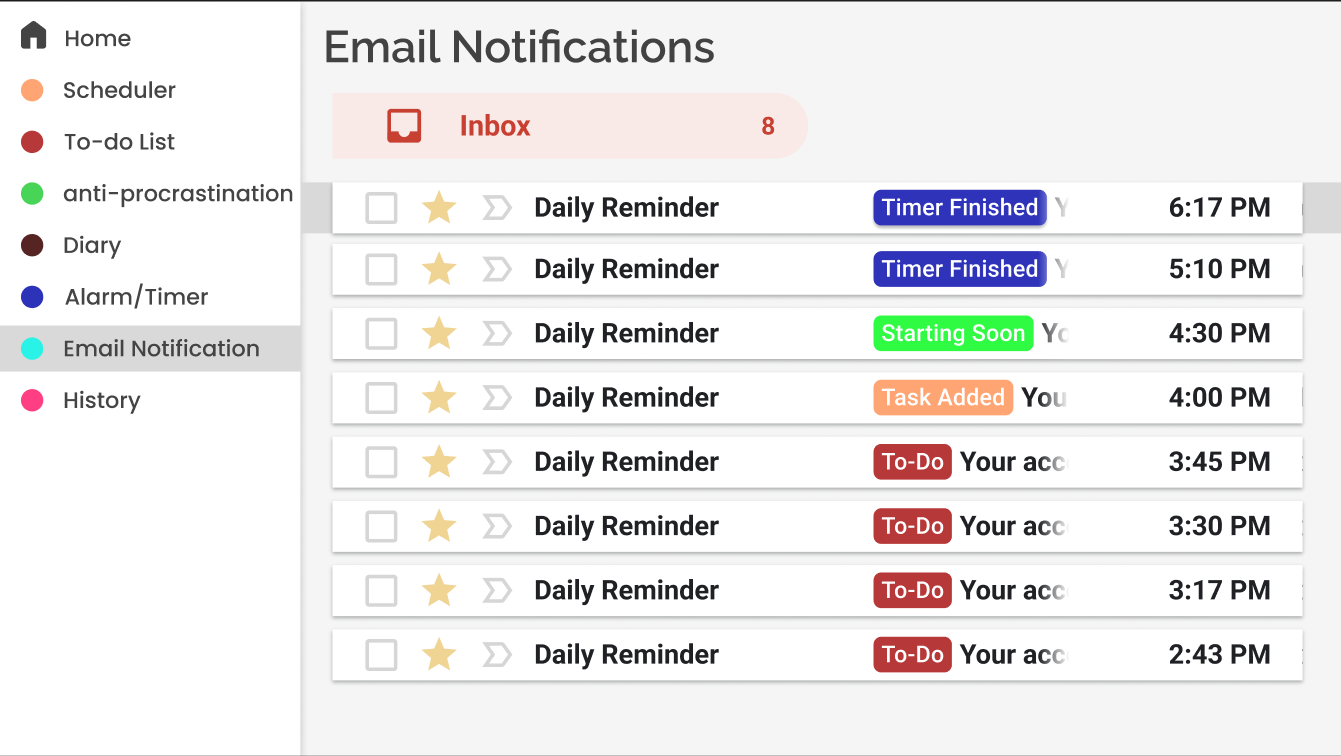
\includegraphics[width=1\textwidth]{./images/Mockup_Email_normal.png}
	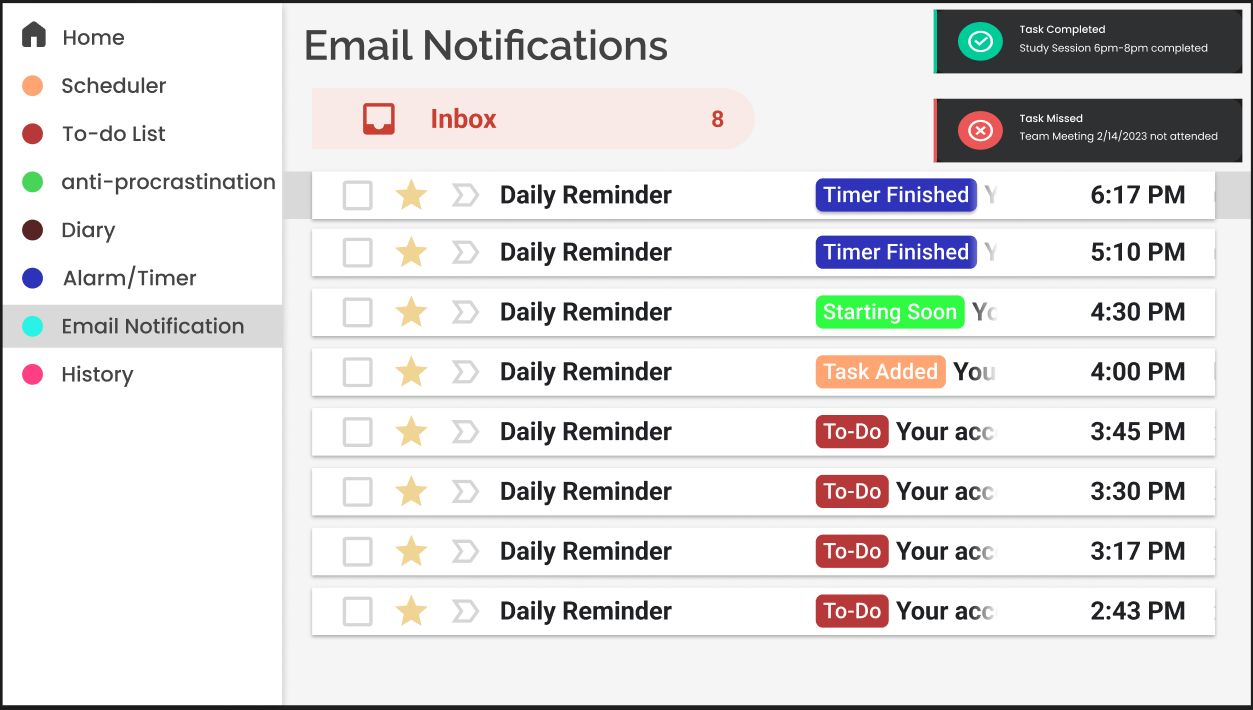
\includegraphics[width=1\textwidth]{./images/Mockup_Email.png} %插入图片,[]中设置图片大小,{}中是图片文件名
	\caption*{Mockup: Email notification} %最终文档中希望显示的图片标题
	\label{Fig.Email} %用于文内引用的标签
\end{figure}

\subsection{Persona}

\begin{figure}[H] %H为当前位置,!htb为忽略美学标准,htbp为浮动图形
	\centering %图片居中
	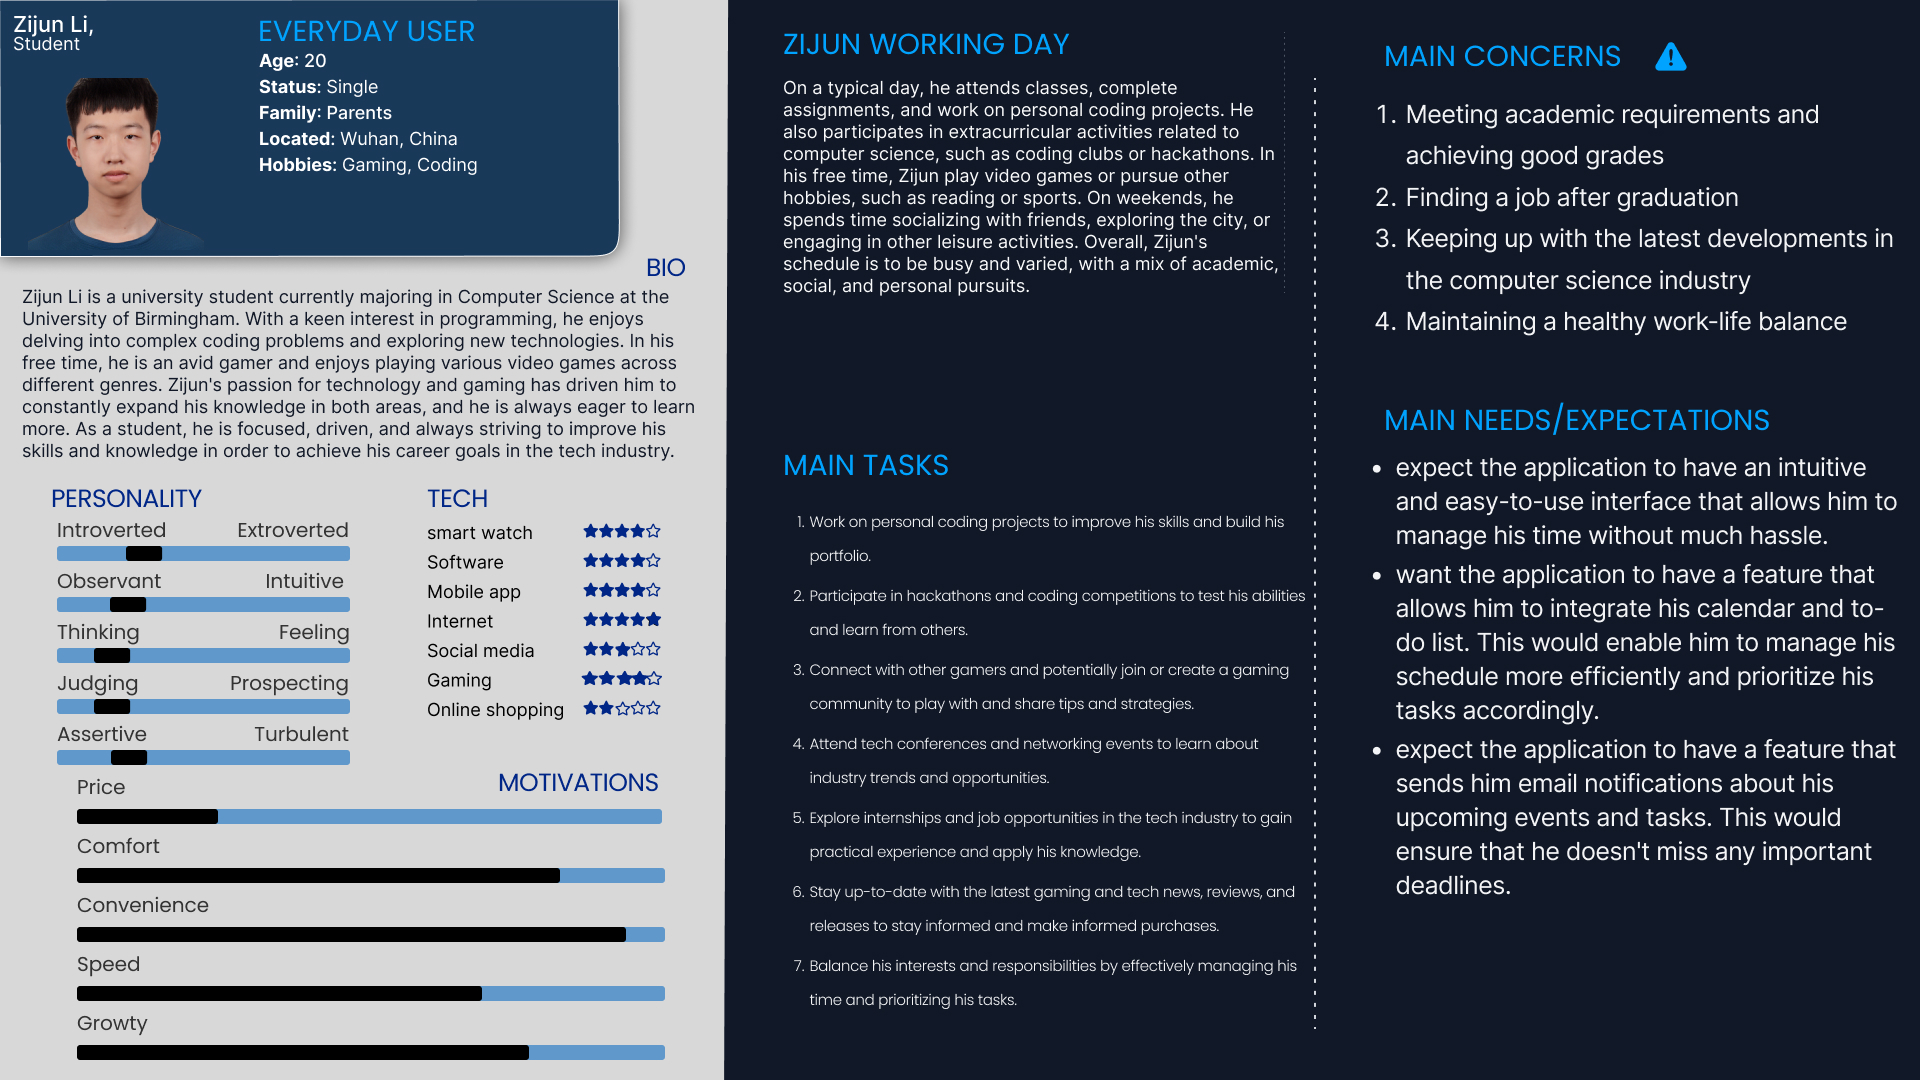
\includegraphics[width=1\textwidth]{./images/Persona_Zijun.jpg} %插入图片,[]中设置图片大小,{}中是图片文件名
	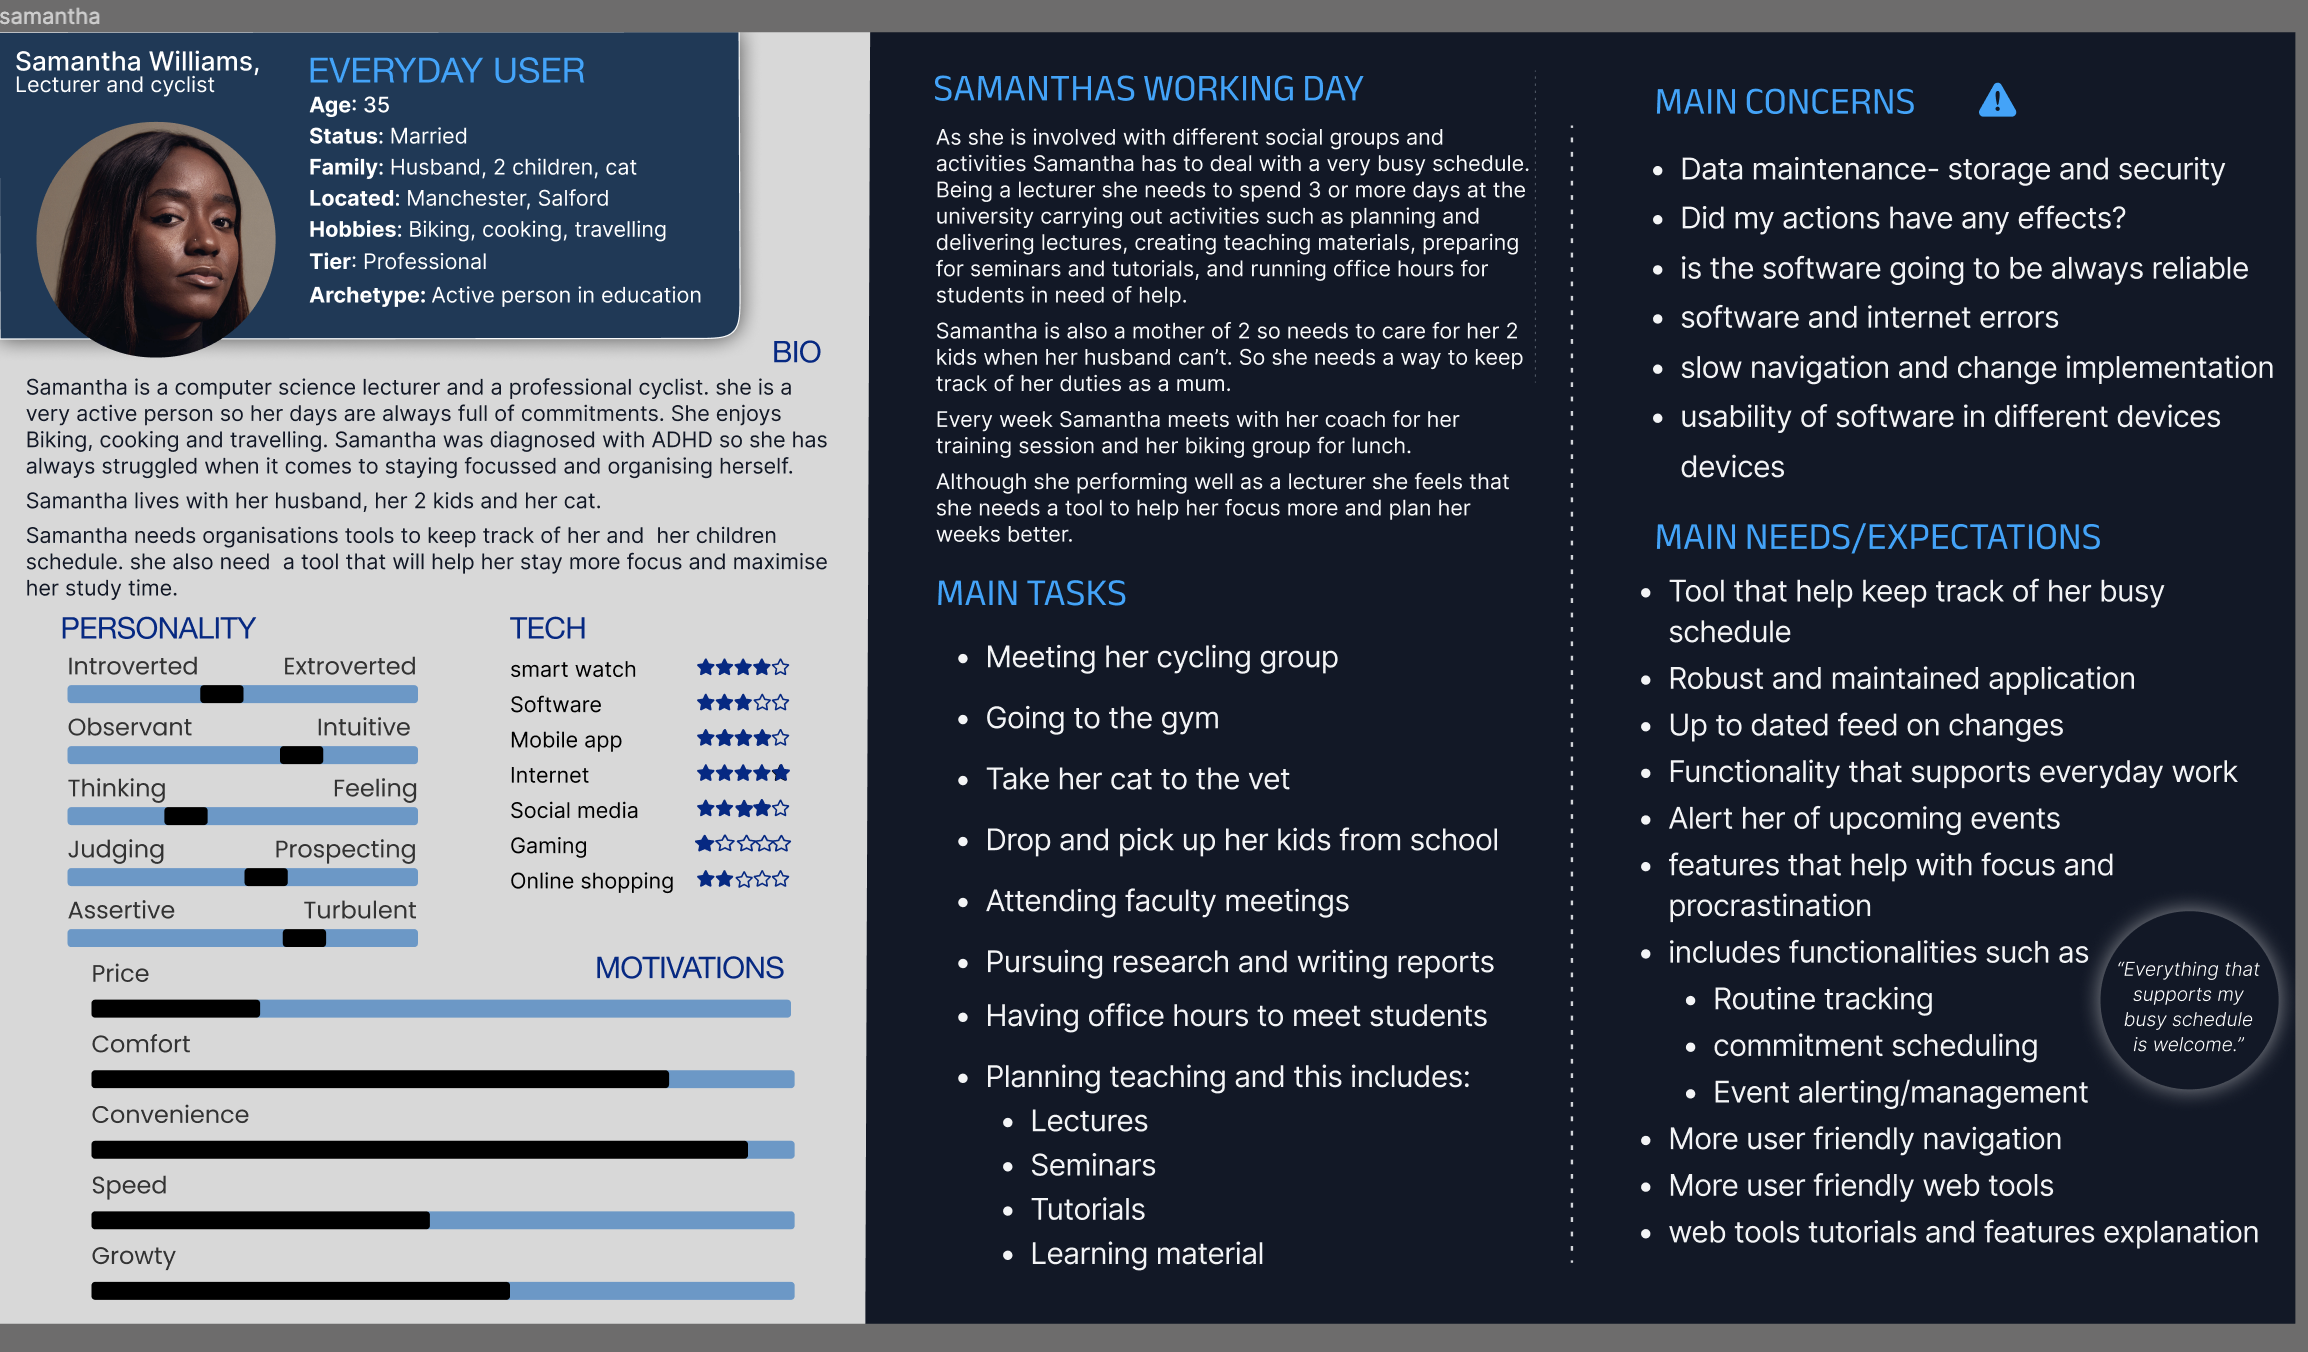
\includegraphics[width=1\textwidth]{./images/Persona_Chance.jpg}
	\caption*{} %最终文档中希望显示的图片标题
	\label{Fig.Personas1} %用于文内引用的标签
\end{figure}

\newpage

\begin{figure}[H] %H为当前位置,!htb为忽略美学标准,htbp为浮动图形
	\centering %图片居中
	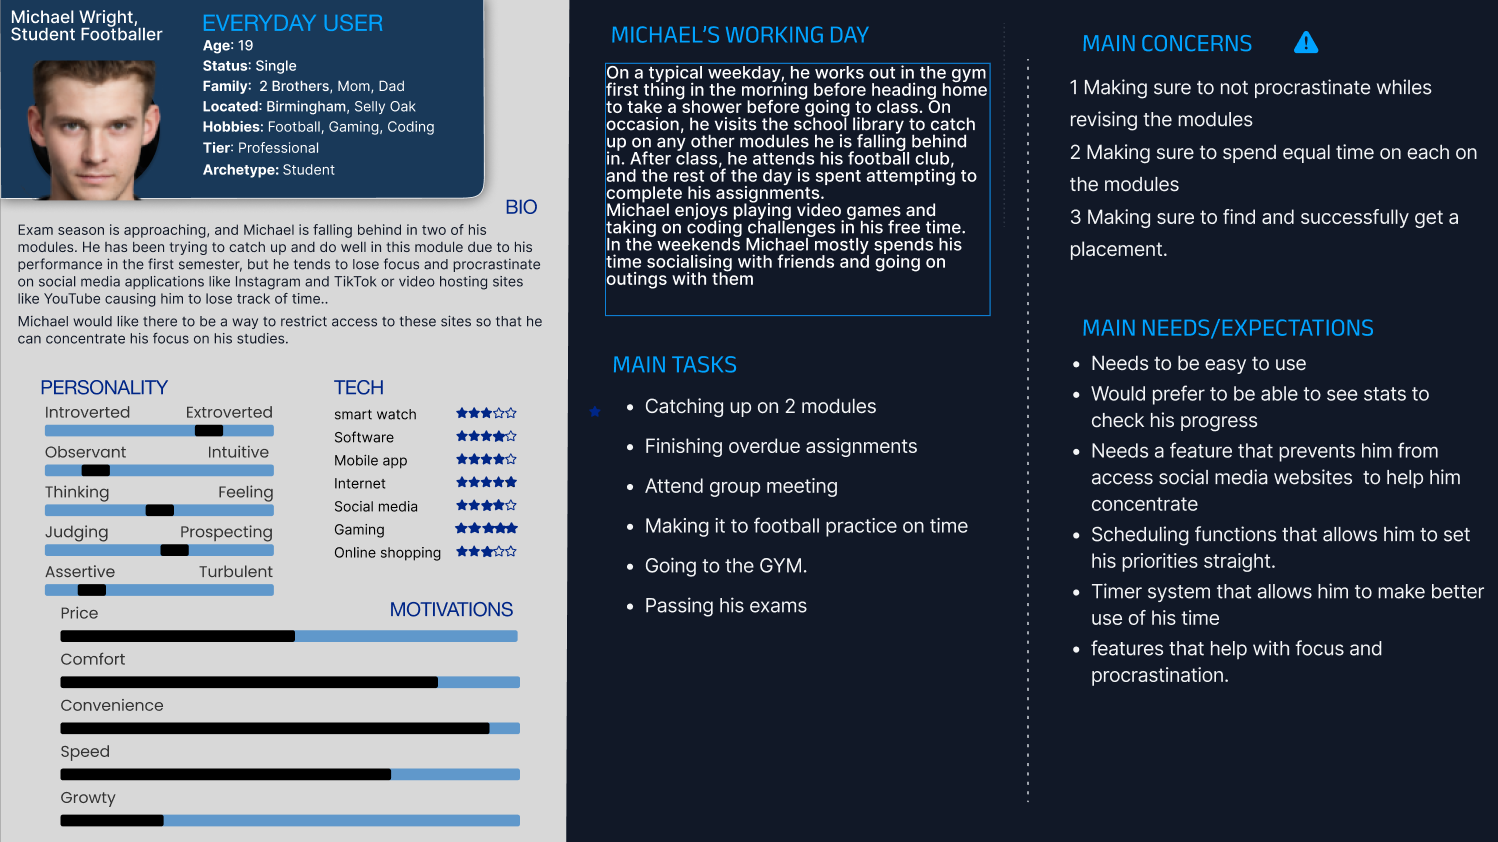
\includegraphics[width=1\textwidth]{./images/Persona_Gilead.png} %插入图片,[]中设置图片大小,{}中是图片文件名
	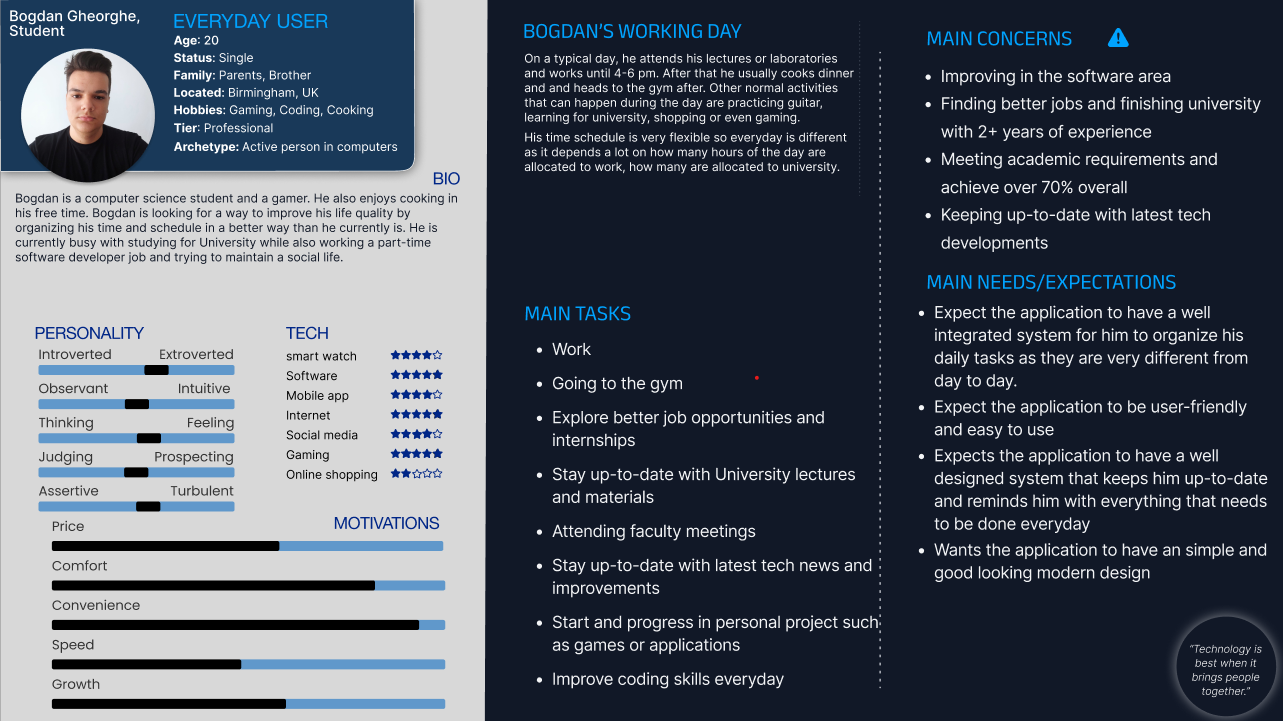
\includegraphics[width=1\textwidth]{./images/Persona_Bogdan.png}
	\caption*{} %最终文档中希望显示的图片标题
	\label{Fig.Persona2} %用于文内引用的标签
\end{figure}

\begin{figure}[H] %H为当前位置,!htb为忽略美学标准,htbp为浮动图形
	\centering %图片居中
	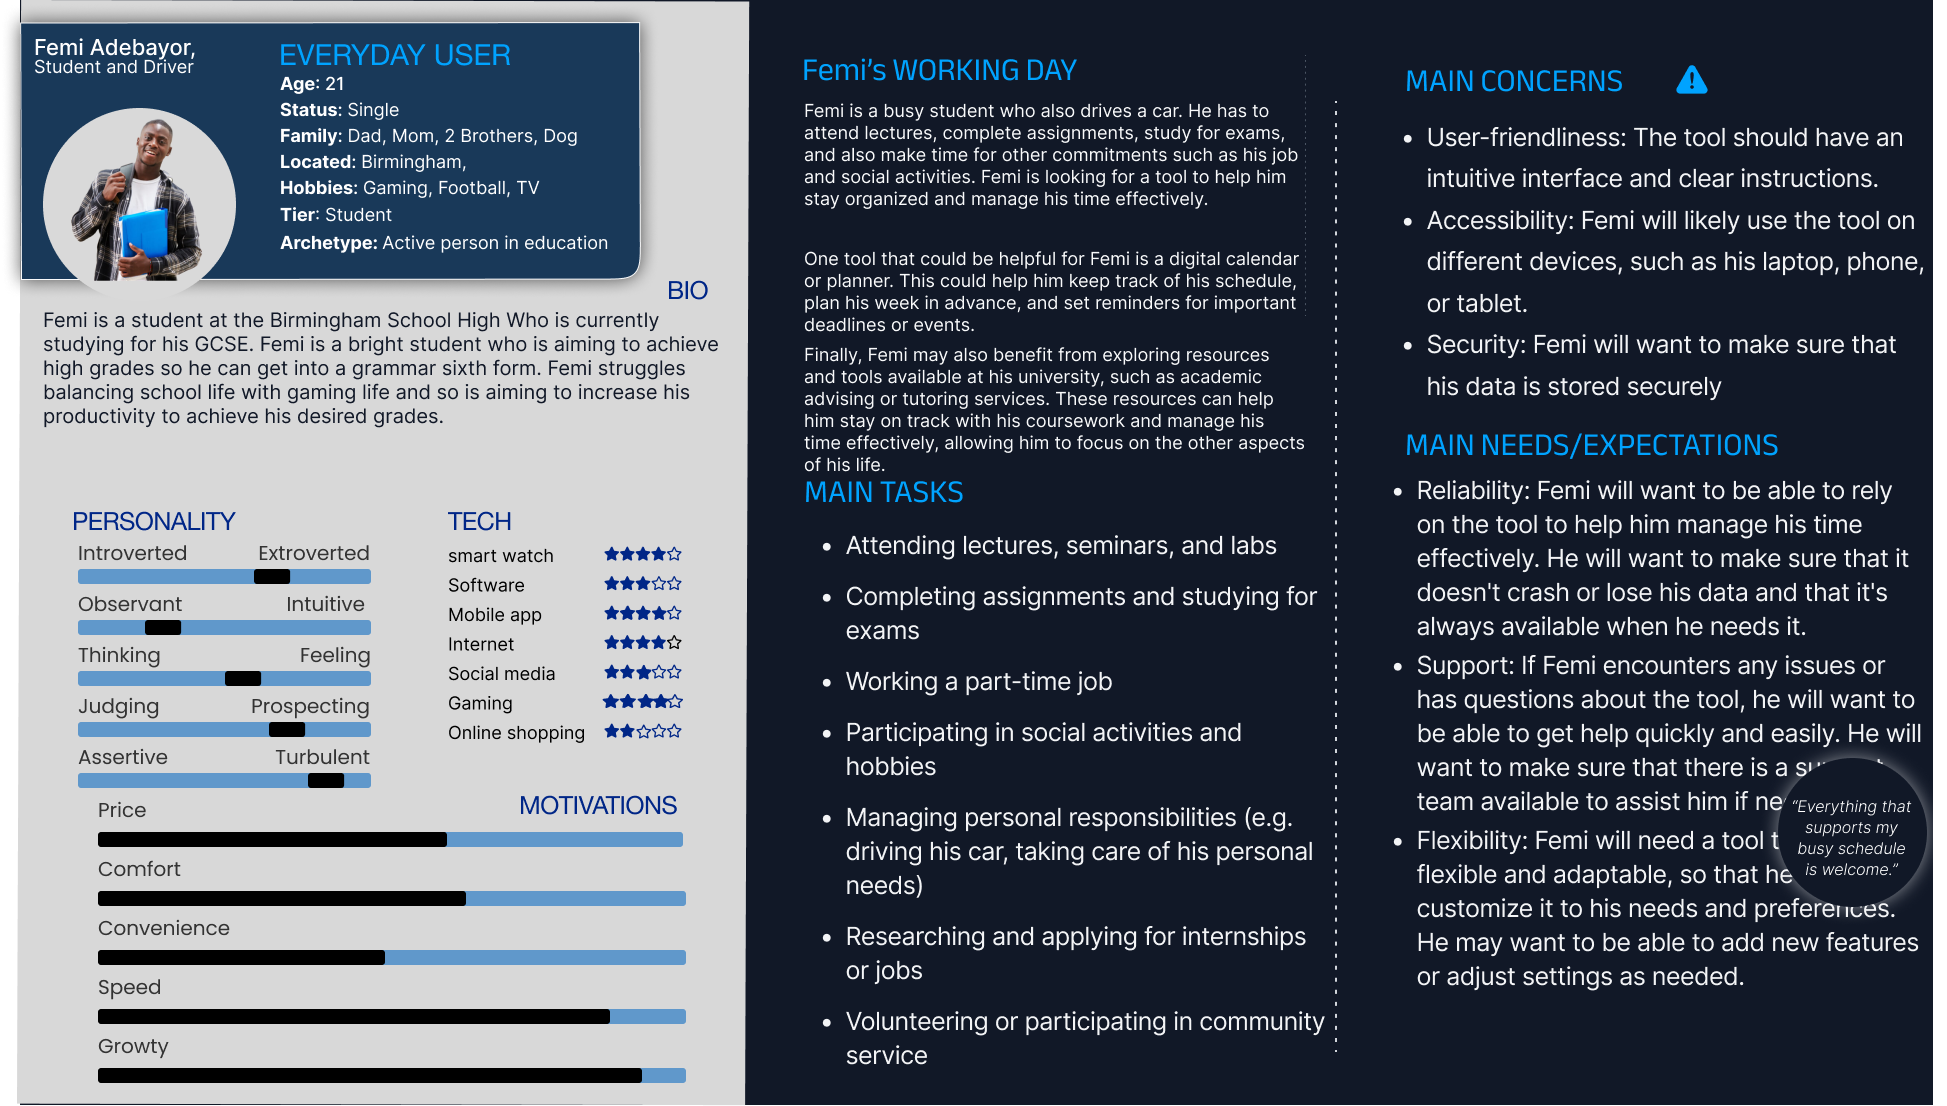
\includegraphics[width=0.92\textwidth]{./images/Persona_Samuel.jpg}
	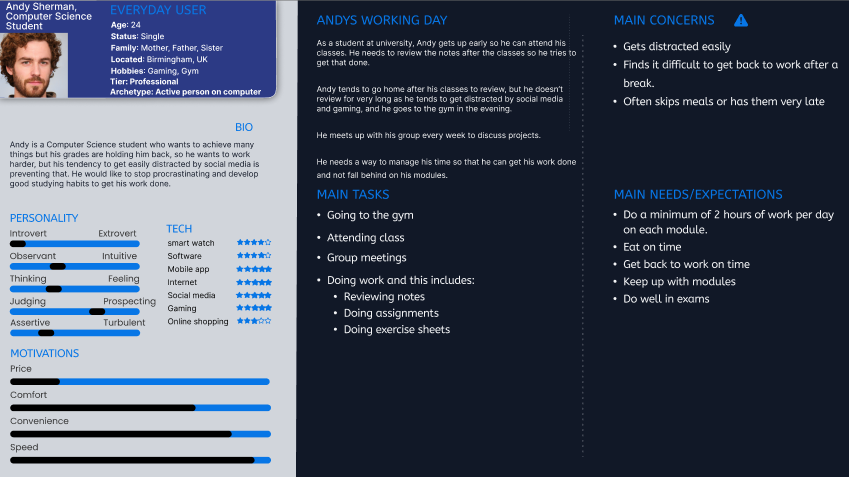
\includegraphics[width=0.92\textwidth]{./images/Persona_Smit.png}
	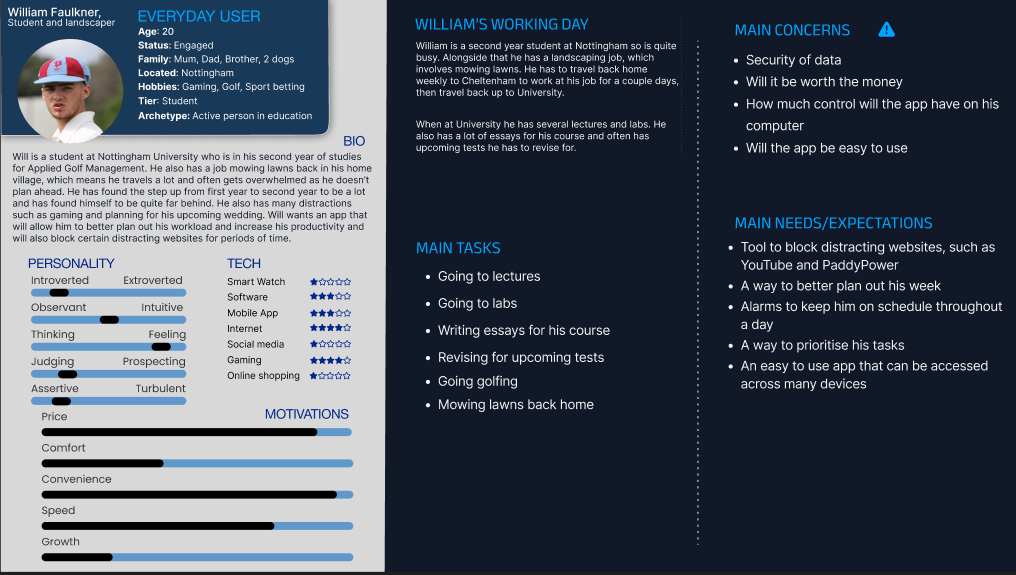
\includegraphics[width=0.92\textwidth]{./images/Persona_Matt.png}
	\caption*{} %最终文档中希望显示的图片标题
	\label{Fig.Persona3} %用于文内引用的标签
\end{figure}

\section{CI pipeline setup}

\begin{figure}[H] %H为当前位置,!htb为忽略美学标准,htbp为浮动图形
	\centering %图片居中
	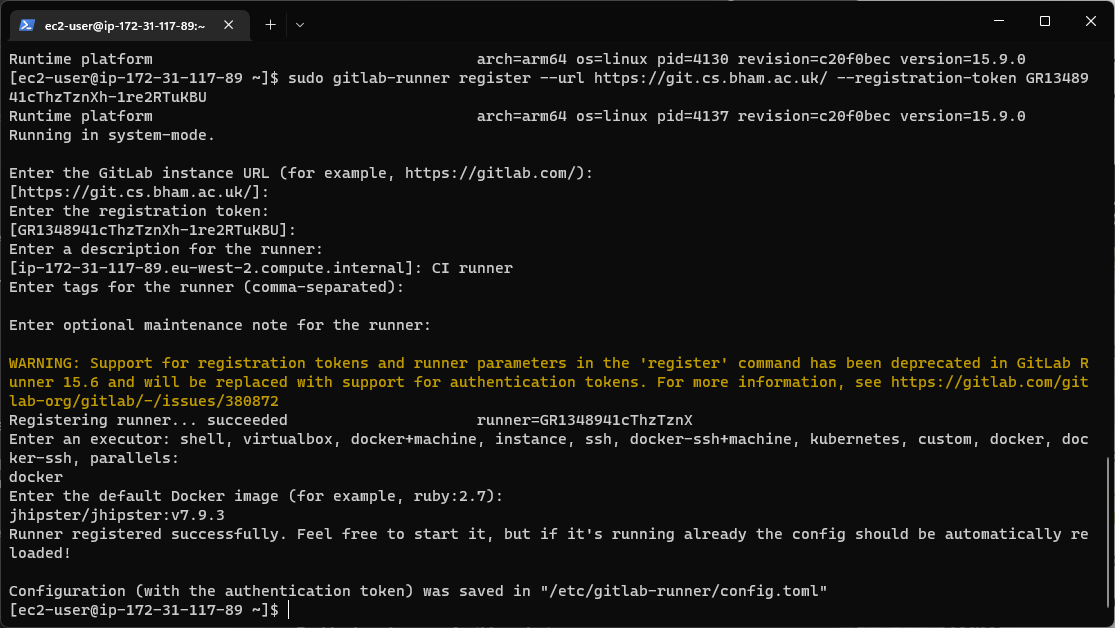
\includegraphics[width=0.84\textwidth]{./images/pipeline_install_gitlab_runner.png}
	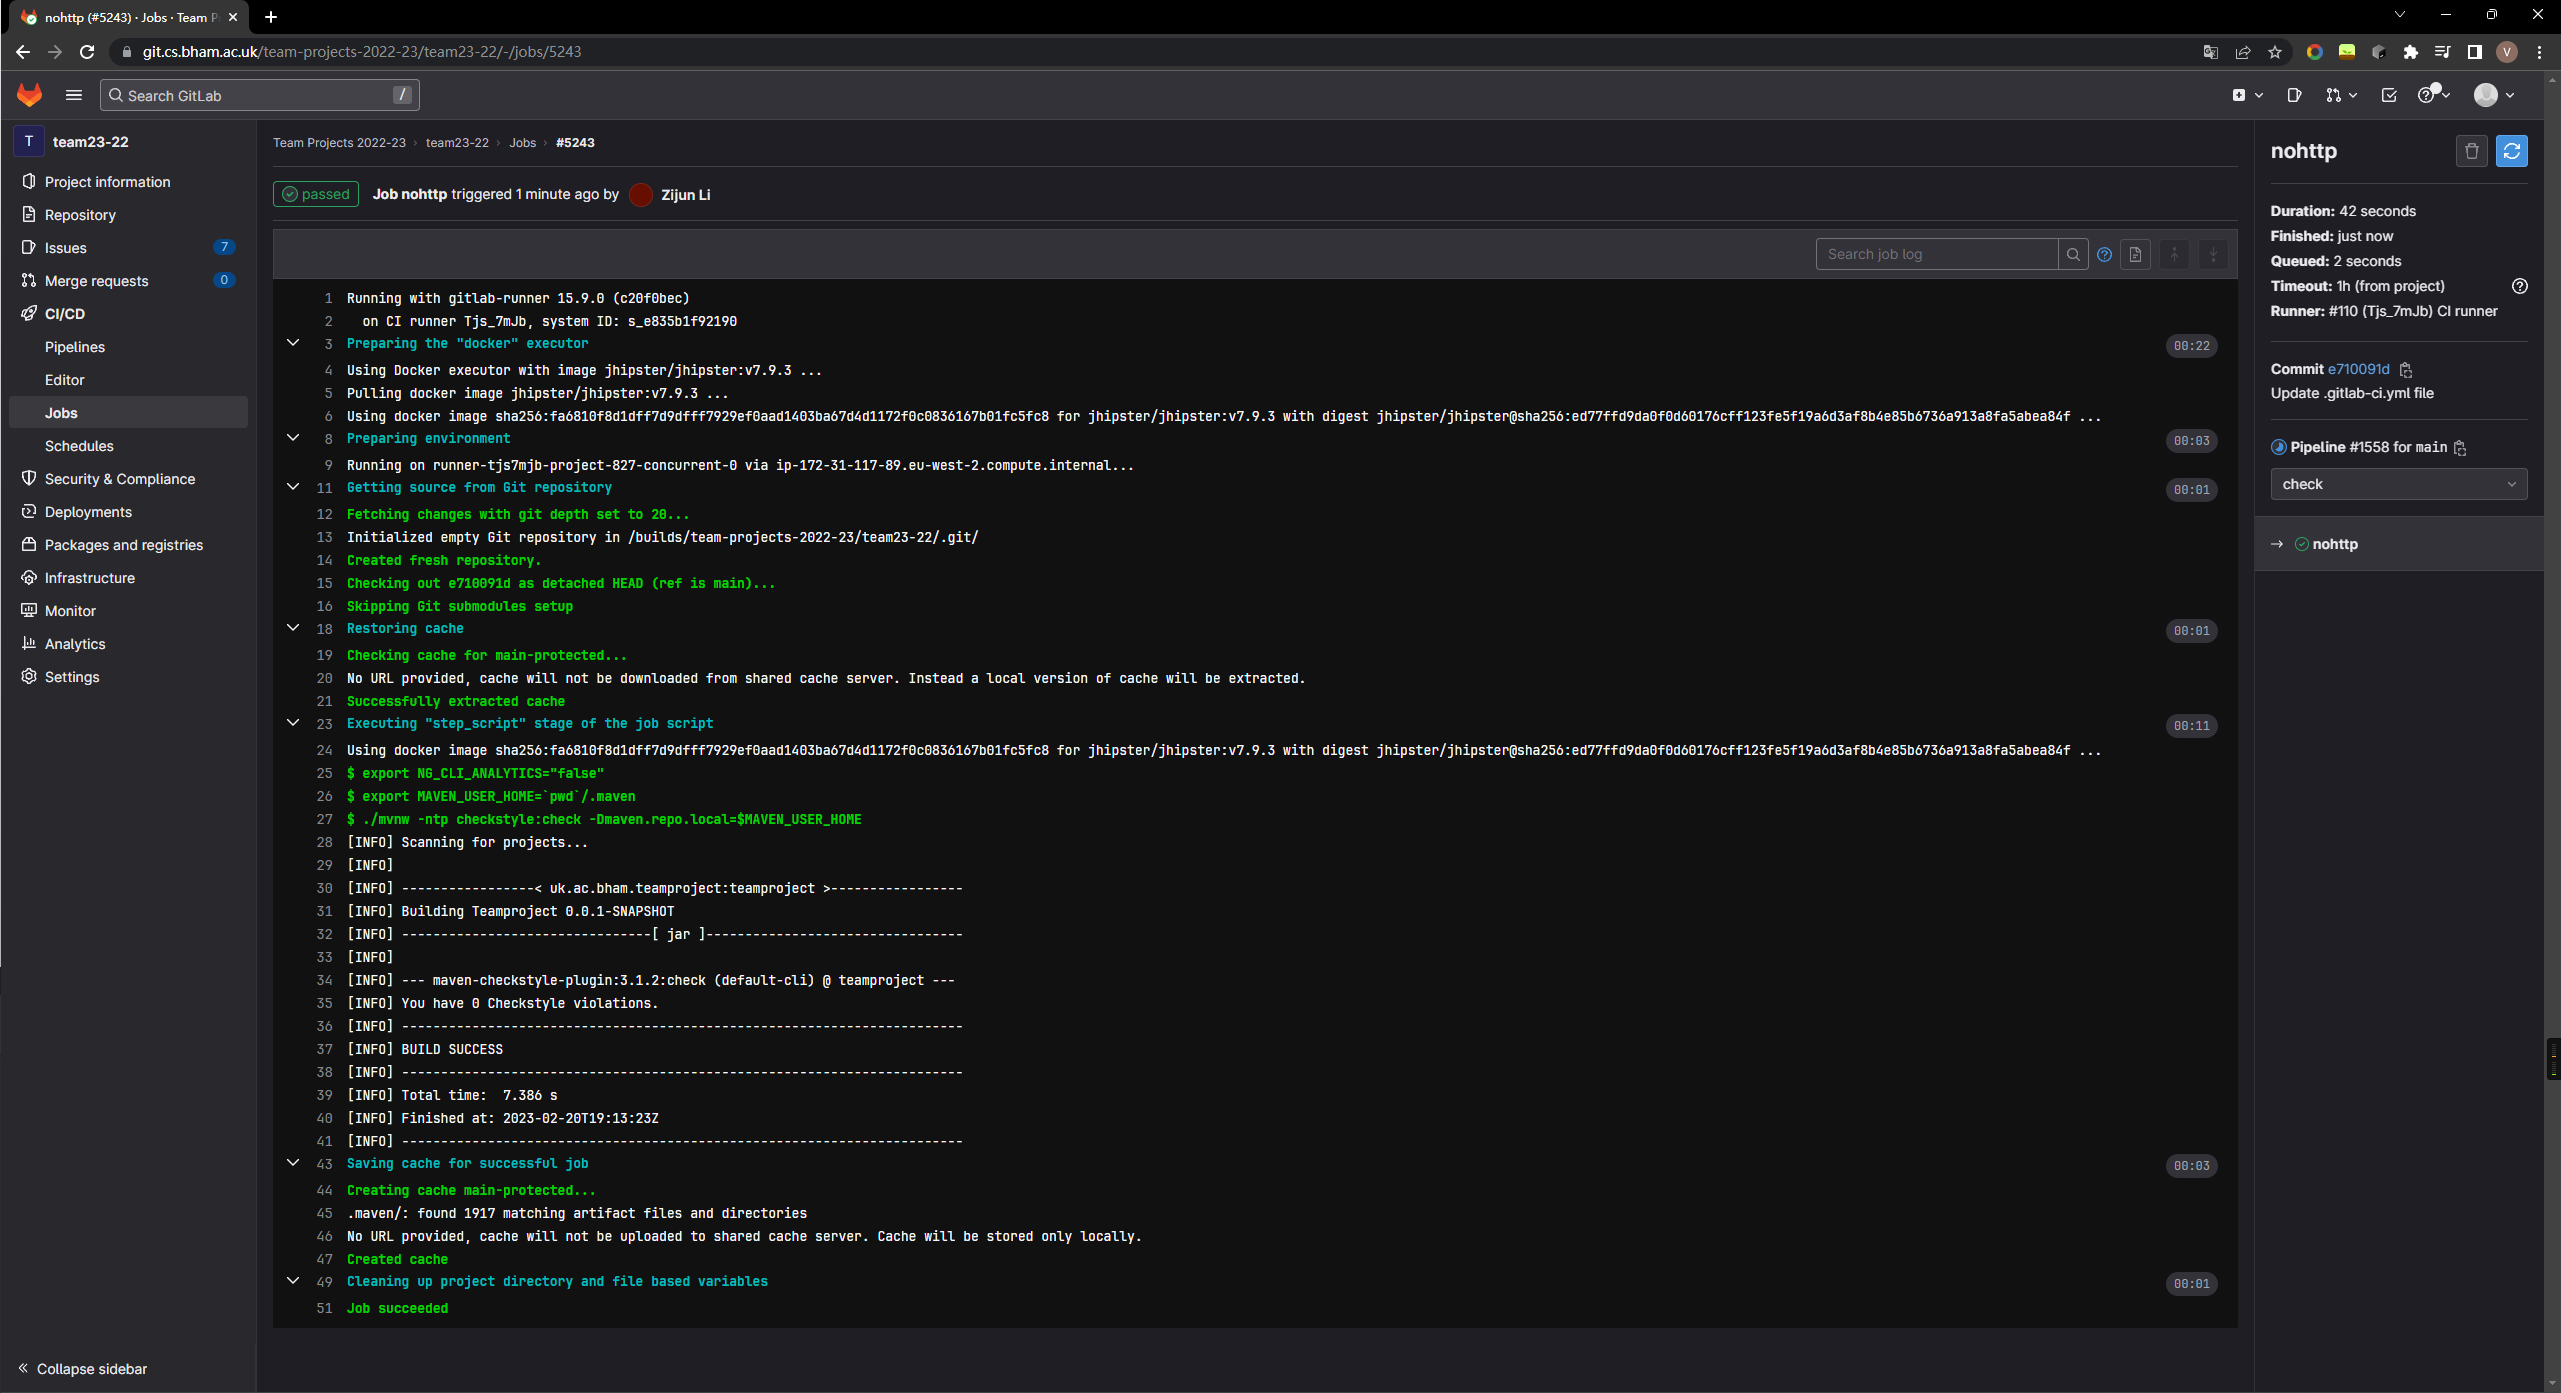
\includegraphics[width=0.84\textwidth]{./images/pipeline_work.png}
	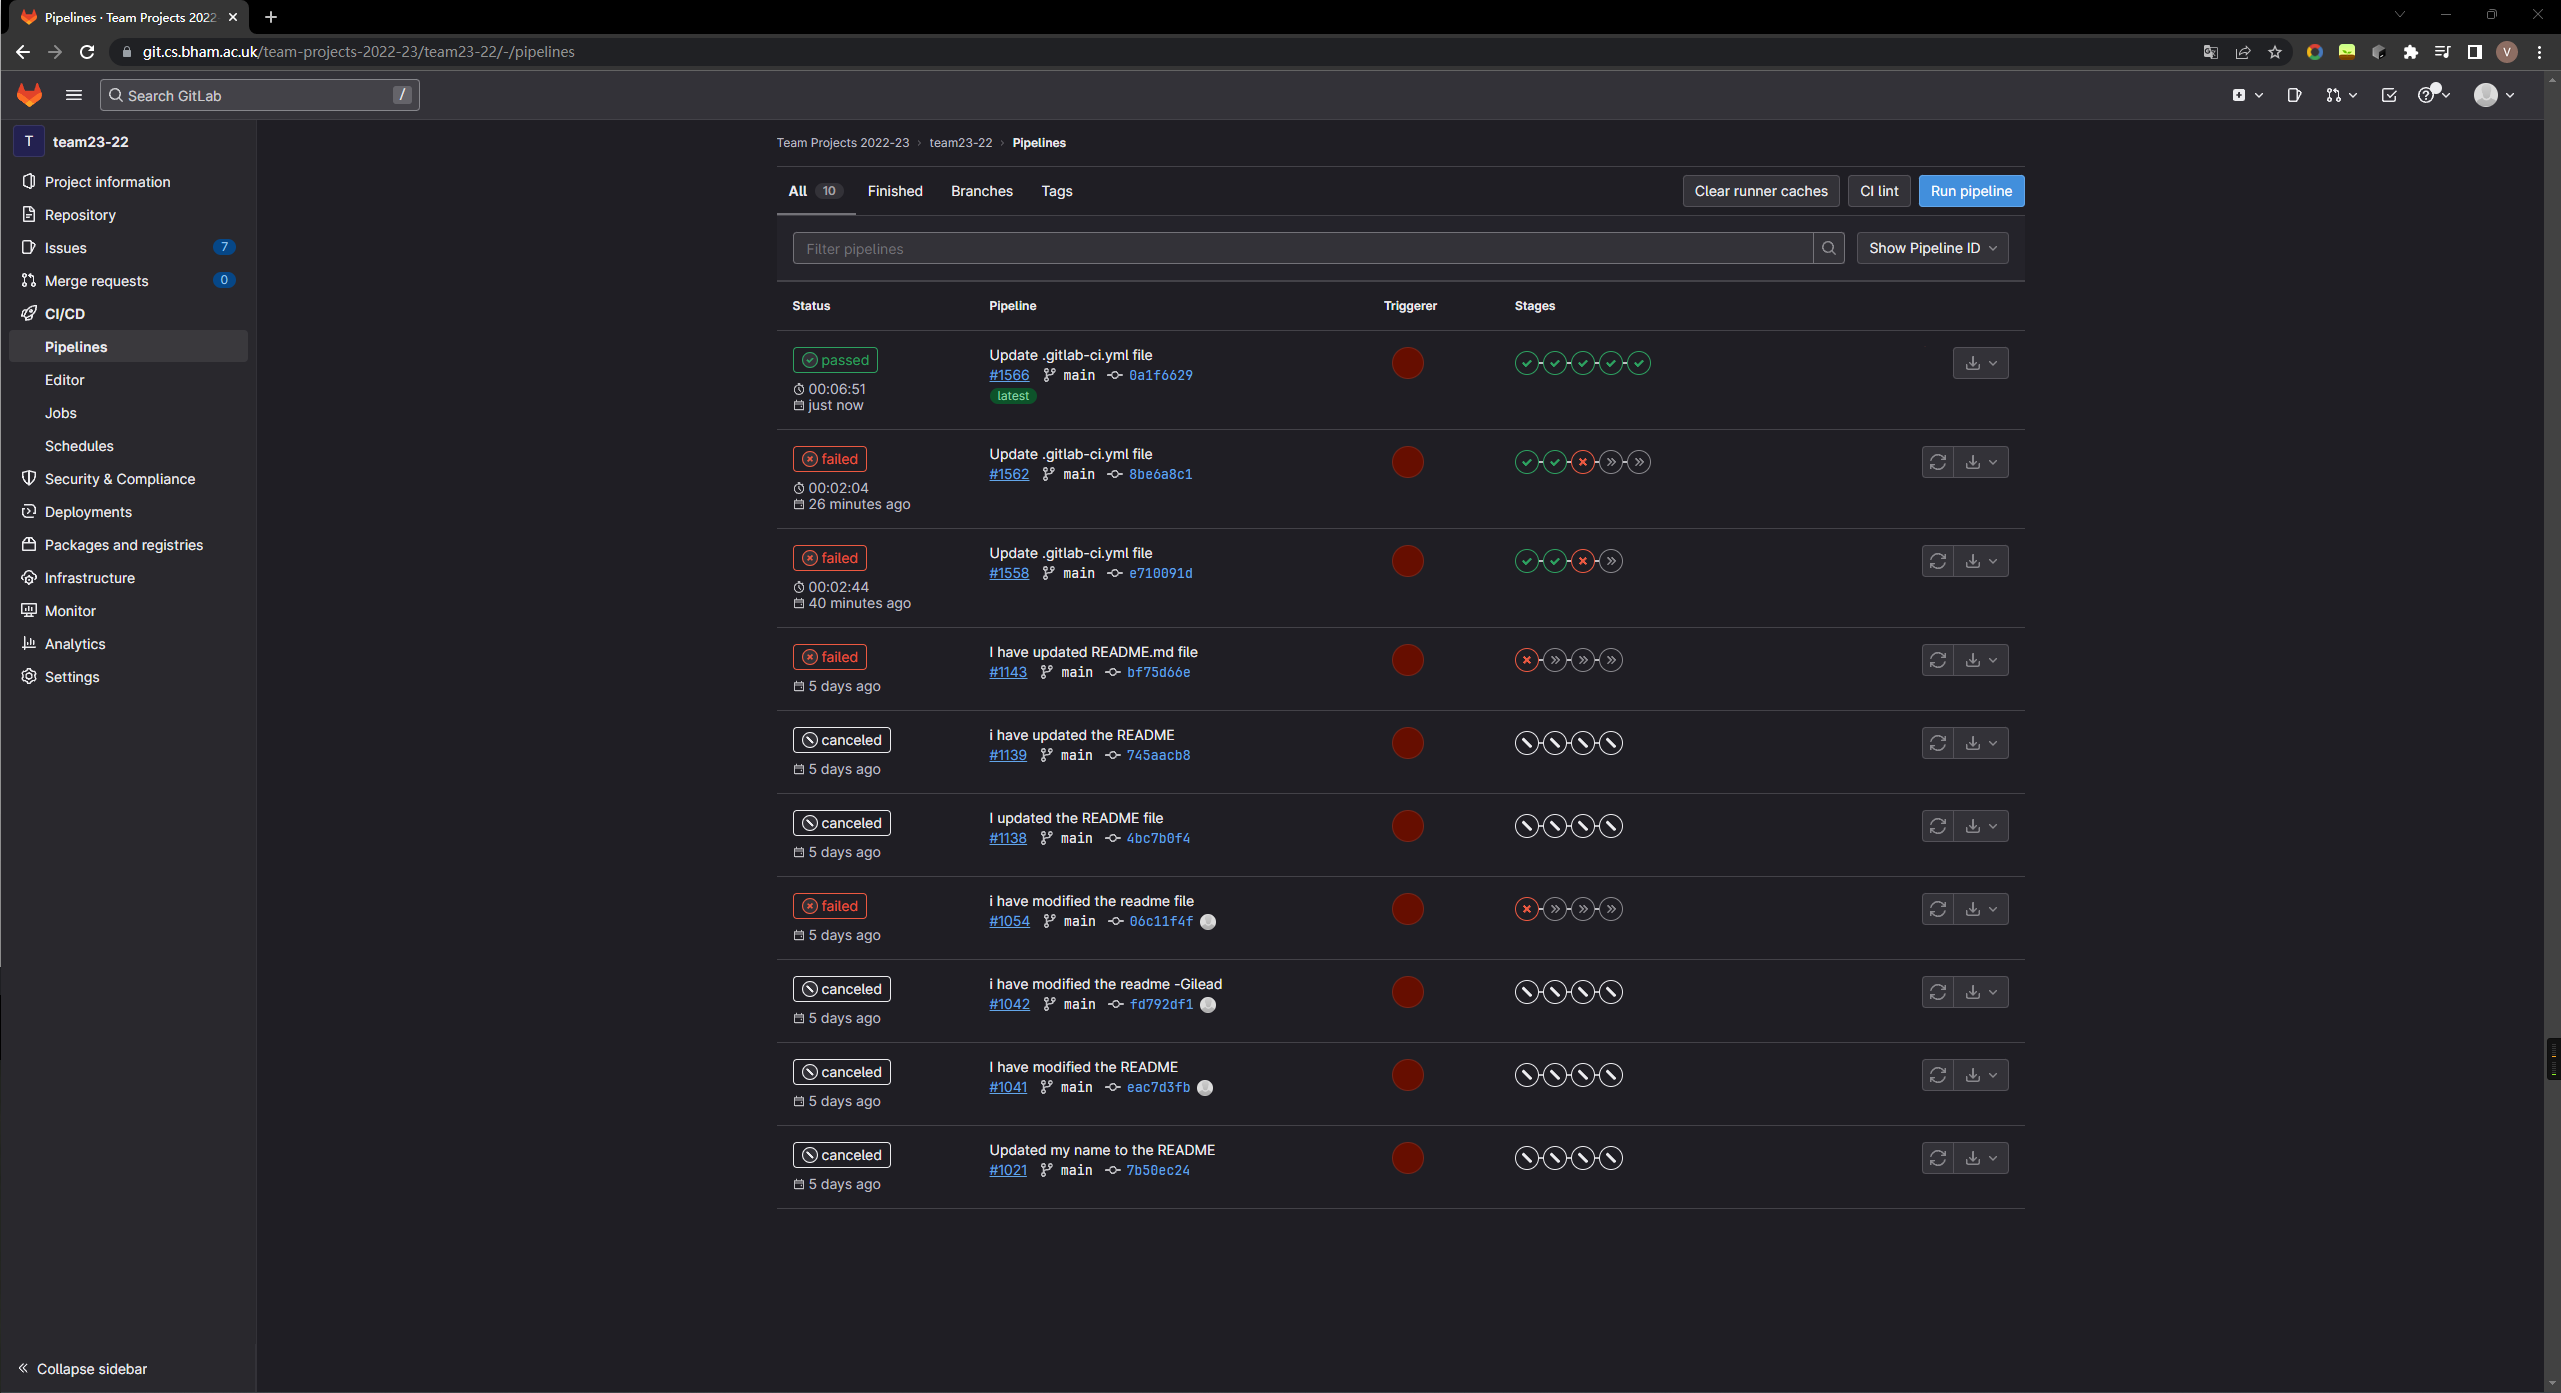
\includegraphics[width=0.84\textwidth]{./images/pipeline_success.png} %插入图片,[]中设置图片大小,{}中是图片文件名
	\caption*{CI pipeline} %最终文档中希望显示的图片标题
	\label{Fig.main2} %用于文内引用的标签
\end{figure}

\newpage

\section{Meeting diary}

{\noindent\begin{tabular}{|p{0.2\linewidth}|p{0.75\linewidth}|} 
	\hline
 \multicolumn{2}{|l|}{\textbf{Week 2: Meeting 1}}\\
 \hline
 \textbf{Date} & 10-2-2023\\
 \hline
 \textbf{Time} & 13:00-13:30(UK Time Zone)\\
 \hline
 \textbf{Venue} & Room 222\\
 \hline
 \multirow{2}*{\textbf{Attendees}} & Meeting Chair: Christian Vergara Marcillo\\
 ~ & Other Participants: Chance Egbon, Gilead Bempah, Matthew Goulding, Zijun Li, Bogdan-Marian Gheorghe\\
 \hline
 \multirow{3}*{\textbf{Discussions}} & - Only one team member was absent from our first meeting with the TA. We asked the TA for more details about the project, such as whether it should be a web application or a mobile application. We also discussed the application's viability, what we would be expected to do for it, and what each team member should submit for the S1. \\
 ~ & - The TA suggested that we combine the Time Management application and the Anti-Procrastination application because their goals were so similar. We also displayed our ideas for our team project application, which included applications for a care home, a murder mystery game, and an anti-procrastination tool. \\
 ~ & - The TA urged us to reduce the scope of the Anti-Procrastination programme to something that might block websites. Originally, we had suggested for the Anti-Procrastination application to be a piece of software that disabled applications on the user's PC until a timer expired. \\
 ~ & - The care home application caught the TA's attention because we suggested that it be both a phone app and a web application, with the website having the full experience and the phone app having less functionality. However, this would have required more work because we are creating both a phone app and a website. \\
 \hline
 \textbf{Decisions Made} & - We decided later in a call that we would put these ideas to a vote with a  form with the highest chosen being the one we would do, and the Anti-Procrastination/Time management application won, we also decided to host regular meetings with each other online using discord to stay up to date with each others progress.\\
 \hline
\end{tabular}}

\hspace*{\fill}\\

{\noindent\begin{tabular}{|p{0.2\linewidth}|p{0.75\linewidth}|} 
	\hline
 \multicolumn{2}{|l|}{\textbf{Week 3: Meeting 1}}\\
 \hline
 \textbf{Date} & 13-2-2023\\
 \hline
 \textbf{Time} & 16:00-16:30(UK Time Zone)\\
 \hline
 \textbf{Venue} & Discord Calls\\
 \hline
 \textbf{Attendees} & Participants: Chance Egbon, Samuel Okasia, Matthew Goulding, Zijun Li, Bogdan-Marian Gheorghe, Gilead Bempah, Smit Navinkumar\\
 \hline
 \multirow{2}*{\textbf{Discussions}} & - At this meeting, we spoke about the features that our application might offer. After coming up with about 7 or 8 features, we divided them up amongst ourselves according to who wanted to work on which feature. \\
 ~ & - We talked about the technology we would use to create our personas and mockups so that some degree of coherence would be achievable, and we then went on to work on our individual mockups for our submissions (Mockup, Persona, Kanban cards, etc...). \\
 \hline
 \textbf{Decisions Made} & - We chose to use the Figma tool for our mockups and Discord as our primary method of communication because it made it simpler for us to assist one another if any problems arose. If someone was having trouble with a particular aspect of S1, we could enter a video call and show our screens to help one another.\\
 \hline
\end{tabular}}

\hspace*{\fill}\\

{\noindent\begin{tabular}{|p{0.2\linewidth}|p{0.75\linewidth}|} 
	\hline
 \multicolumn{2}{|l|}{\textbf{Week 3: Meeting 2}}\\
 \hline
 \textbf{Date} & 14-2-2023\\
 \hline
 \textbf{Time} & 14:20-14:40(UK Time Zone)\\
 \hline
 \textbf{Venue} & Room 117\\
 \hline
 \multirow{2}*{\textbf{Attendees}} & Meeting Chair: Christian Vergara Marcillo \\
 ~ & Other Participants: Chance Egbon, Samuel Okasia, Matthew Goulding, Zijun Li, Bogdan-Marian Gheorghe \\
 \hline
 \textbf{Discussions} & - During the meeting, we asked TA for suggestions on the format of the mockups and personas.\\
 \hline
 \textbf{Decisions Made} & - TA provided some useful insights, including emphasizing the importance of including more detailed information in personas to make them more useful and realistic. The suggestion was also made to use standard templates for both mockups and personas to ensure consistency and clarity.\\
 \hline
\end{tabular}}

\hspace*{\fill}\\

{\noindent\begin{tabular}{|p{0.2\linewidth}|p{0.75\linewidth}|} 
	\hline
 \multicolumn{2}{|l|}{\textbf{Week 4: Meeting 1}}\\
 \hline
 \textbf{Date} & \makecell[l]{21-2-2023}\\
 \hline
 \textbf{Time} & \makecell[l]{14:20-14:40(UK Time Zone)}\\
 \hline
 \textbf{Venue} & \makecell[l]{Room 225}\\
 \hline
 \multirow{2}*{\textbf{Attendees}} & Meeting Chair: Christian Vergara Marcillo \\
 ~ & Other Participants: Matthew Goulding, Zijun Li, Smit Navinkumar, Gilead Bempah \\
 \hline
 \multirow{2}*{\textbf{Discussions}} & - We discussed the M1 team assessment during this meeting, and the TA provided more information about what we needed to complete before submitting. In particular, he spoke to us about our mockups and how we would need to remake them to be coherent with one another. He also advised us to start developing (coding) our application as soon as possible because it will give us more time to fix any errors we discover. He also suggested that we collaborate and determine among ourselves which database application we would utilise for our application. \\
 ~ & - We talked about how we would accomplish these goals after the meeting was over. \\
 \hline
 \textbf{Decisions Made} & - We changed the persona and mockup styles to the ones that received the greatest scores in the S1 ranking.\\
 \hline
\end{tabular}}

\section{S2 task allocation \& planning}

\subsection{Scheduler}

\begin{figure}[H] %H为当前位置,!htb为忽略美学标准,htbp为浮动图形
	\centering %图片居中
	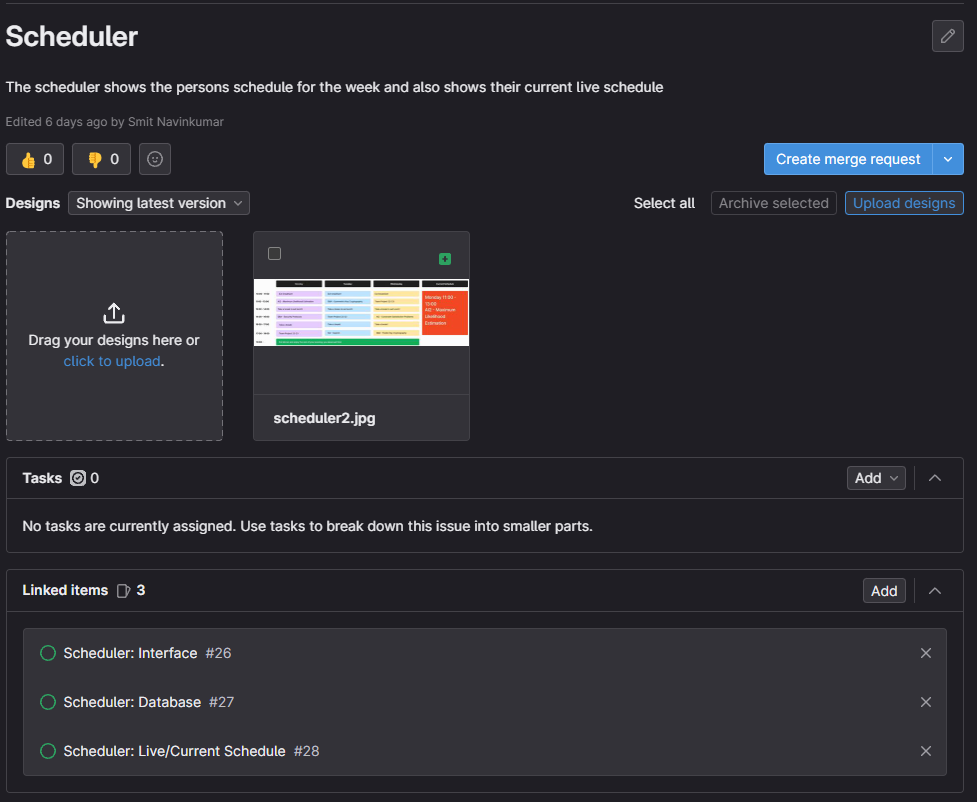
\includegraphics[width=0.85\textwidth]{./images/S2_Scheduler.png}
	\caption*{Smit} %最终文档中希望显示的图片标题
	\label{Fig.S2_Scheduler} %用于文内引用的标签
\end{figure}

\subsection{To-do List}

\begin{figure}[H] %H为当前位置,!htb为忽略美学标准,htbp为浮动图形
	\centering %图片居中
	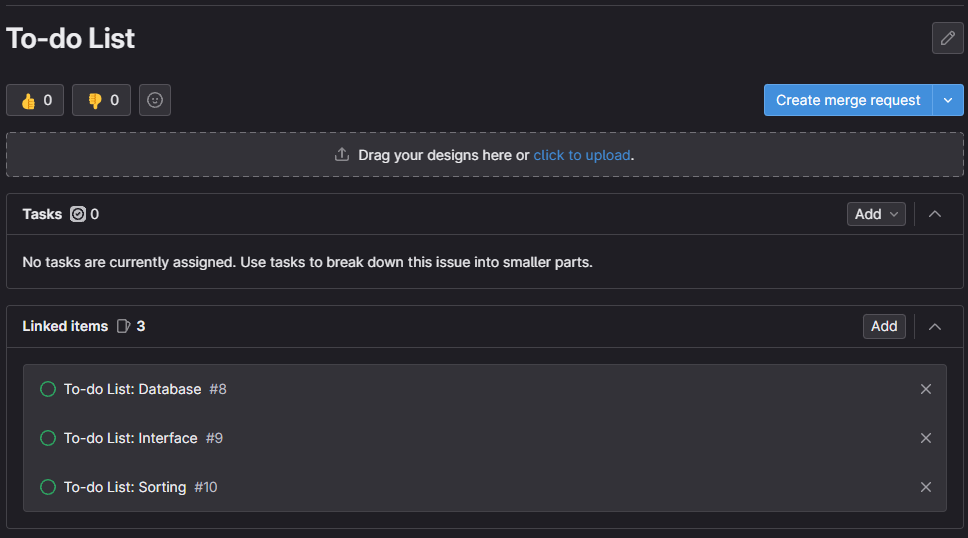
\includegraphics[width=0.85\textwidth]{./images/S2_To-do_List.png}
	\caption*{Zijun} %最终文档中希望显示的图片标题
	\label{Fig.S2_todo} %用于文内引用的标签
\end{figure}

\subsection{Anti-procrastination}

\begin{figure}[H] %H为当前位置,!htb为忽略美学标准,htbp为浮动图形
	\centering %图片居中
	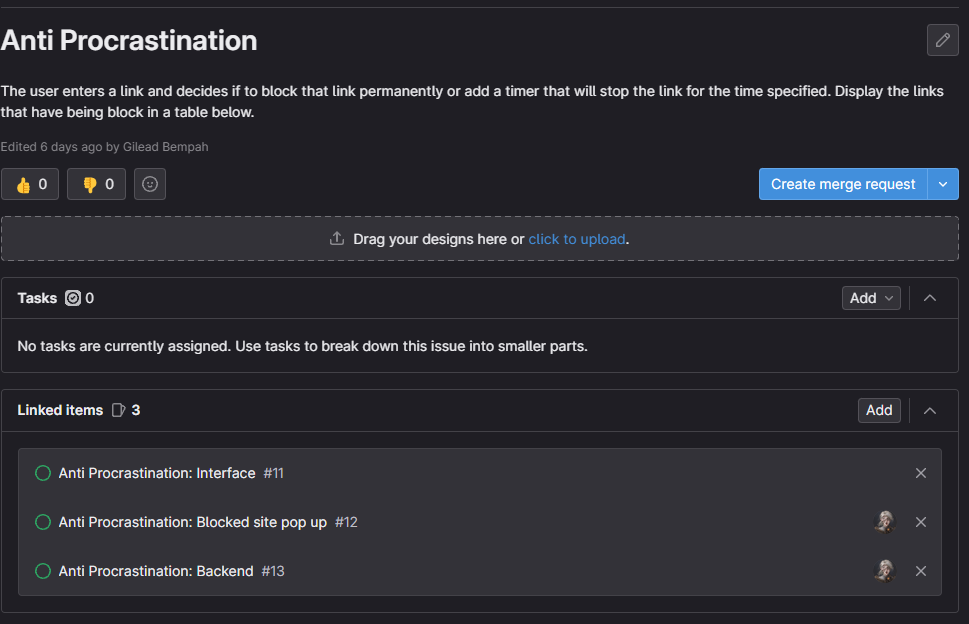
\includegraphics[width=0.85\textwidth]{./images/S2_Anti-Procrastination.png}
	\caption*{Gilead} %最终文档中希望显示的图片标题
	\label{Fig.S2_Anti-procrastination} %用于文内引用的标签
\end{figure}

\subsection{Diary}

\begin{figure}[H] %H为当前位置,!htb为忽略美学标准,htbp为浮动图形
	\centering %图片居中
	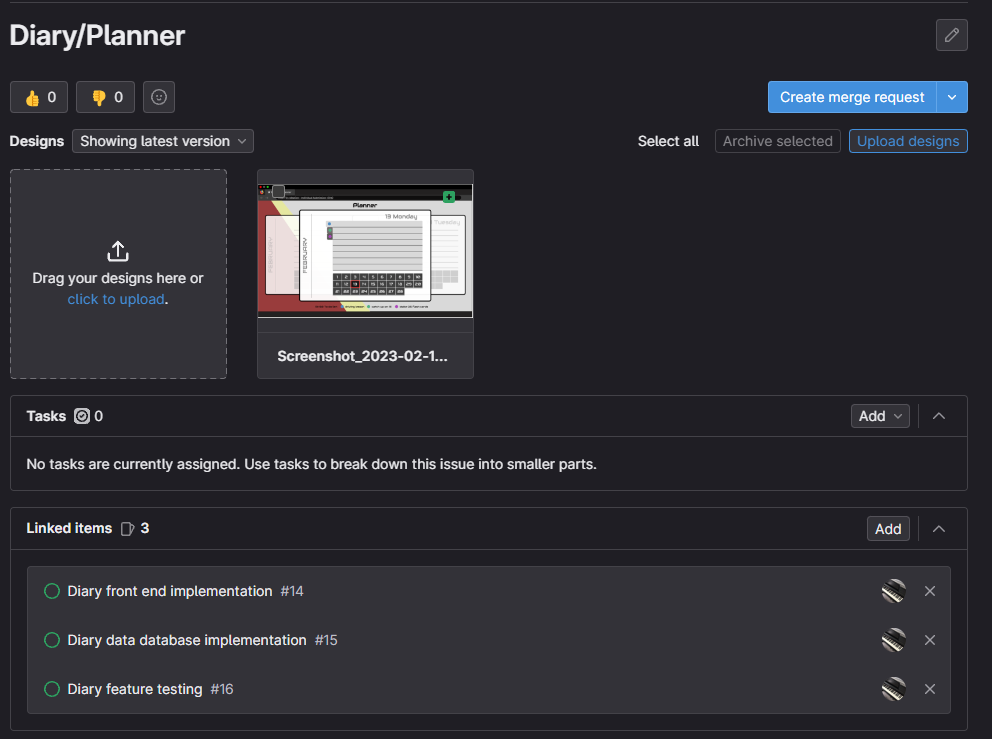
\includegraphics[width=0.85\textwidth]{./images/S2_Diary.png}
	\caption*{Chance} %最终文档中希望显示的图片标题
	\label{Fig.S2_Diary} %用于文内引用的标签
\end{figure}

\subsection{Alarm/Timer}

\begin{figure}[H] %H为当前位置,!htb为忽略美学标准,htbp为浮动图形
	\centering %图片居中
	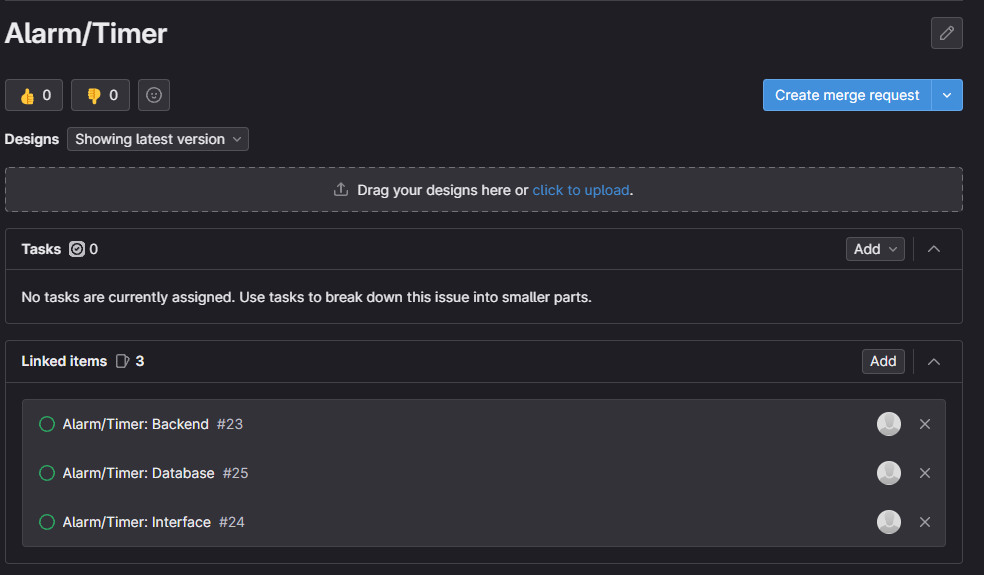
\includegraphics[width=0.76\textwidth]{./images/S2_Alarm.png}
	\caption*{Matthew} %最终文档中希望显示的图片标题
	\label{Fig.S2_Alarm} %用于文内引用的标签
\end{figure}

\subsection{Email notifications}

\begin{figure}[H] %H为当前位置,!htb为忽略美学标准,htbp为浮动图形
	\centering %图片居中
	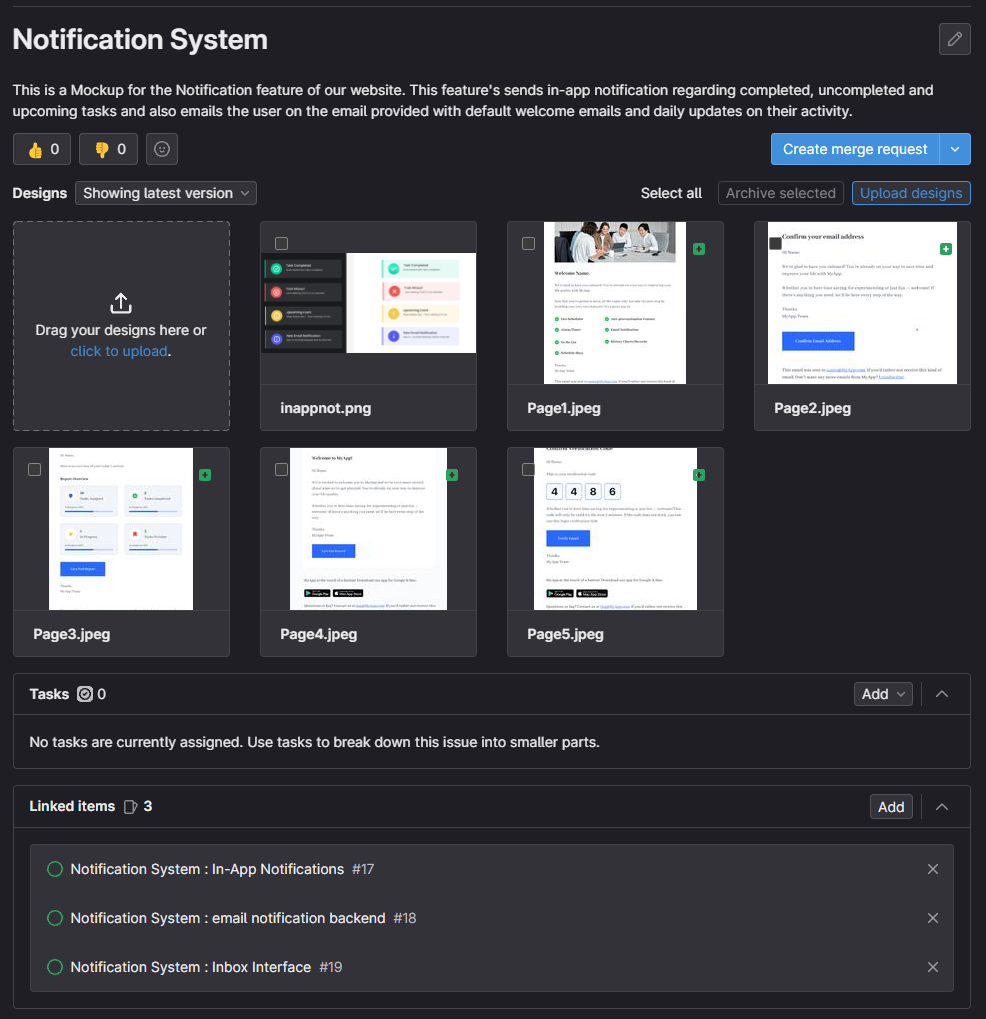
\includegraphics[width=0.76\textwidth]{./images/S2_Email.png}
	\caption*{Bogdan} %最终文档中希望显示的图片标题
	\label{Fig.S2_Email} %用于文内引用的标签
\end{figure}

\subsection{History}

\begin{figure}[H] %H为当前位置,!htb为忽略美学标准,htbp为浮动图形
	\centering %图片居中
	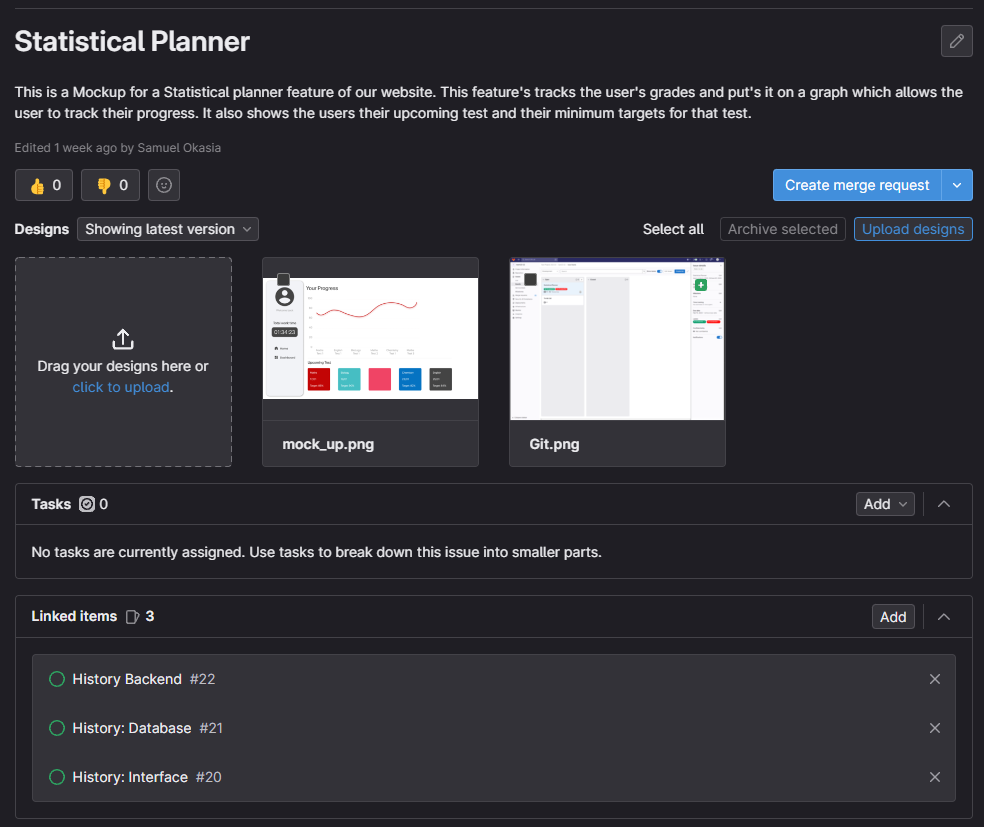
\includegraphics[width=0.85\textwidth]{./images/S2_History.png}
	\caption*{Samuel} %最终文档中希望显示的图片标题
	\label{Fig.S2_History} %用于文内引用的标签
\end{figure}

\end{document}